\PassOptionsToPackage{dvipsnames}{xcolor}
\PassOptionsToPackage{hyphens}{url}
\documentclass[referee,lineno,pdflatex,sn-nature]{sn-jnl}
\usepackage{graphicx}
\usepackage{microtype}
\usepackage{environ}
\usepackage{booktabs}
\usepackage{multirow}
\usepackage{tabularx}
\usepackage{placeins}
\usepackage{xr}
\externaldocument[S-]{supplementary}
\usepackage{amsmath}
\usepackage{amssymb}
\usepackage{mathtools}
\usepackage{tikz}
\usetikzlibrary{arrows.meta, positioning, calc, fit, shapes.geometric, backgrounds, decorations.pathreplacing}
\hypersetup{hidelinks,bookmarksdepth=2}

\setcounter{secnumdepth}{2}
\raggedbottom
\emergencystretch=2em
\setlength{\textfloatsep}{12pt plus 2pt minus 2pt}
\setlength{\floatsep}{12pt plus 2pt minus 2pt}
\setlength{\intextsep}{12pt plus 2pt minus 2pt}
\setlength{\abovecaptionskip}{6pt}
\setlength{\belowcaptionskip}{4pt}

\NewEnviron{deferredmethodsintro}{\global\let\deferredmethodsintrobody\BODY}
\NewEnviron{deferredmethodsrest}{\global\let\deferredmethodsrestbody\BODY}
\NewEnviron{deferredmethoddetails}{\global\let\deferredmethoddetailsbody\BODY}
\NewEnviron{deferreddiscussion}{\global\let\deferreddiscussionbody\BODY}

\IfFileExists{main_metrics_v2.tex}{%
  % Generated from validated matched-v2 full-year metrics.
\newcommand{\WBSixRMSE}{0.06263}
\newcommand{\WBSixDCAERMSE}{0.07075}
\newcommand{\WBSixLinearRMSE}{0.12680}
\newcommand{\WBSixVsLinearGainPct}{50.6}
\newcommand{\WBSixSeenRMSE}{0.05484}
\newcommand{\WBSixHeldRMSE}{0.07431}
\newcommand{\WBSixDCAEHeldRMSE}{0.08167}
\newcommand{\WBSixLinearHeldRMSE}{0.14445}
\newcommand{\WBSixHeldVsDCAEGainPct}{9.0}
\newcommand{\WBSixHeldVsLinearGainPct}{48.6}
\newcommand{\WBTwelveRMSE}{0.10812}
\newcommand{\WBTwelveDCAERMSE}{0.11654}
\newcommand{\WBTwelveLinearRMSE}{0.22265}
\newcommand{\WBTwelveSeenRMSE}{0.09888}
\newcommand{\WBTwelveHeldRMSE}{0.13277}
\newcommand{\WBTwelveDCAEHeldRMSE}{0.14098}
\newcommand{\WBTwelveLinearHeldRMSE}{0.27820}
\newcommand{\WBTwelveVsLinearHeldGainPct}{52.3}
\newcommand{\WBTwelveHeldVsDCAEGainPct}{5.8}
\newcommand{\WBTwelveVsLinearGainPct}{51.4}
\newcommand{\WBTwelveACC}{0.98660}
\newcommand{\WBTwelveHeldACC}{0.98110}
%
}{}

\IfFileExists{case_metrics_v2.tex}{%
  % Auto-generated by tools/eval/export_case_metrics_tex.py.
\newcommand{\WBHaishenLinearTauThree}{0.793}
\newcommand{\WBHaishenWeatherBridgeTauThree}{0.383}
\newcommand{\WBHaishenLinearMean}{0.610}
\newcommand{\WBHaishenWeatherBridgeMean}{0.336}
\newcommand{\WBIdaLinearTauThree}{1.078}
\newcommand{\WBIdaWeatherBridgeTauThree}{0.664}
\newcommand{\WBIdaLinearMean}{0.849}
\newcommand{\WBIdaWeatherBridgeMean}{0.572}
\newcommand{\WBIdaTruthMax}{30.2}
\newcommand{\WBIdaTruthMaxLat}{29.38}
\newcommand{\WBIdaTruthMaxLon}{270.6}
\newcommand{\WBIdaLinearPeakError}{-9.5}
\newcommand{\WBIdaWeatherBridgePeakError}{-7.3}
%
}{}

\title[WeatherBridge interpolation]{WeatherBridge and the limits of global weather interpolation at held-out query times}

\author*[1,2]{\fnm{Daniil} \sur{Sukhorukov}}
\email{suhorukov.dan0@gmail.com}
\author[1]{\fnm{Andrei} \sur{Zakharov}}
\author[3]{\fnm{Yuri} \sur{Maximov}}
\author[1,4]{\fnm{Ilya} \sur{Makarov}}
\author[1]{\fnm{Ivan} \sur{Oseledets}}
\affil[1]{\orgname{AI Research Institute},
\orgaddress{\city{Moscow}, \country{Russia}}}
\affil[2]{\orgname{AI Talent Hub, ITMO University},
\orgaddress{\city{Saint Petersburg}, \country{Russia}}}
\affil[3]{\orgname{International Center for Corporate Data Analysis},
\orgaddress{\city{Astana}, \country{Kazakhstan}}}
\affil[4]{\orgname{Trusted AI Center, RAS},
\orgaddress{\city{Moscow}, \country{Russia}}}

\abstract{Many forecast archives provide six-hourly fields, but applications
need hourly states. We ask whether a learned interpolator can
recover intermediate trajectories from two endpoints at query hours omitted
from training. We compare linear interpolation and six architectures at
six- and twelve-hour horizons, and test transfer to IFS HRES forecasts.
A matched six-hour WeatherBridge control receives supervision at every interior
hour. WeatherBridge combines
query-conditioned bidirectional transport with multiscale and spectral
corrections. It has the lowest aggregate error at held-out query hours at both
horizons, although no model wins every field. The matched control improves
held-out query hours but barely changes trained ones, measuring the cost of
withholding query times. Models trained on ERA5 lose this advantage
on forecast trajectories; HRES adaptation recovers about 7\% over linear
interpolation in a retrospective audit.
Learned interpolation captures nonlinear motion and small-scale structure
between sparse anchors, while temporal coverage and anchor-domain mismatch
bound its benefit.}

\keywords{weather interpolation, held-out query times, IFS HRES, anchor
transport, ERA5}

\begin{document}

\maketitle

\section{Introduction}

Global forecast archives and benchmarks commonly expose states on fixed
temporal grids. GraphCast predicts at six-hour intervals
\cite{lam2023graphcast}, whereas Pangu-Weather includes separate one-, three-,
six- and 24-hour models \cite{bi2022pangu}. FuXi, Aurora, Stormer, AIFS and
GenCast provide further examples of learned global forecast systems
\cite{chen2023fuxi,bodnar2024aurora,nguyen2024stormer,moldovan2026aifs,price2024genwc}.
FourCastNet uses Fourier operators for global prediction
\cite{kurth2023fourcastnet}, while NeuralGCM learns components of a numerical
general circulation model \cite{kochkov2024neuralgcm}. ClimaX trains a
foundation model spanning weather and climate tasks
\cite{nguyen2023climax}. FengWu extends skilful deterministic forecasts
beyond a ten-day lead for selected fields \cite{chen2025fengwu}, while
Aardvark predicts weather directly from observations
\cite{allen2025aardvark}. Keisler demonstrated an early global
graph-network forecaster \cite{keisler2022gnn}.
WeatherBench and
WeatherBench~2 provide shared forecast-verification protocols
\cite{rasp2020weatherbench,rasp2024weatherbench}.
ERA5 provides hourly reference states \cite{hersbach2020era5}. Recovering an interior state
$x_\tau$ from known anchors $x_0$ and $x_T$ is an interpolation problem, not
a forecast: information from the later anchor is available by definition.
Linear interpolation is consequently a strong reference, but it assumes that
each Eulerian grid value follows the chord between its endpoint values. A
translated pressure system, moisture filament or near-surface wind feature
does not obey that assumption. Its amplitude can be attenuated even when the
two anchors resolve the feature clearly.
Motion-aware reconstruction has precedents in optical-flow precipitation
nowcasting \cite{bowler2004interpolation,pulkkinen2019pysteps} and, more
broadly, in the characteristic-based transport used by semi-Lagrangian
atmospheric schemes \cite{staniforth1991semi}.

Figure~\ref{fig:graphical_overview} shows the interpolation task and the
target-dependent training loop. The interior ERA5 state provides supervision
during training and the reference during evaluation; inference uses only the
two anchors and query metadata. We use 2020 for development, 2021 for calendar
transfer and a prespecified 2022 ERA5 sample for a later calendar check.
Methods records the complete split and HRES development chronology.

\begin{figure}[!t]
\centering
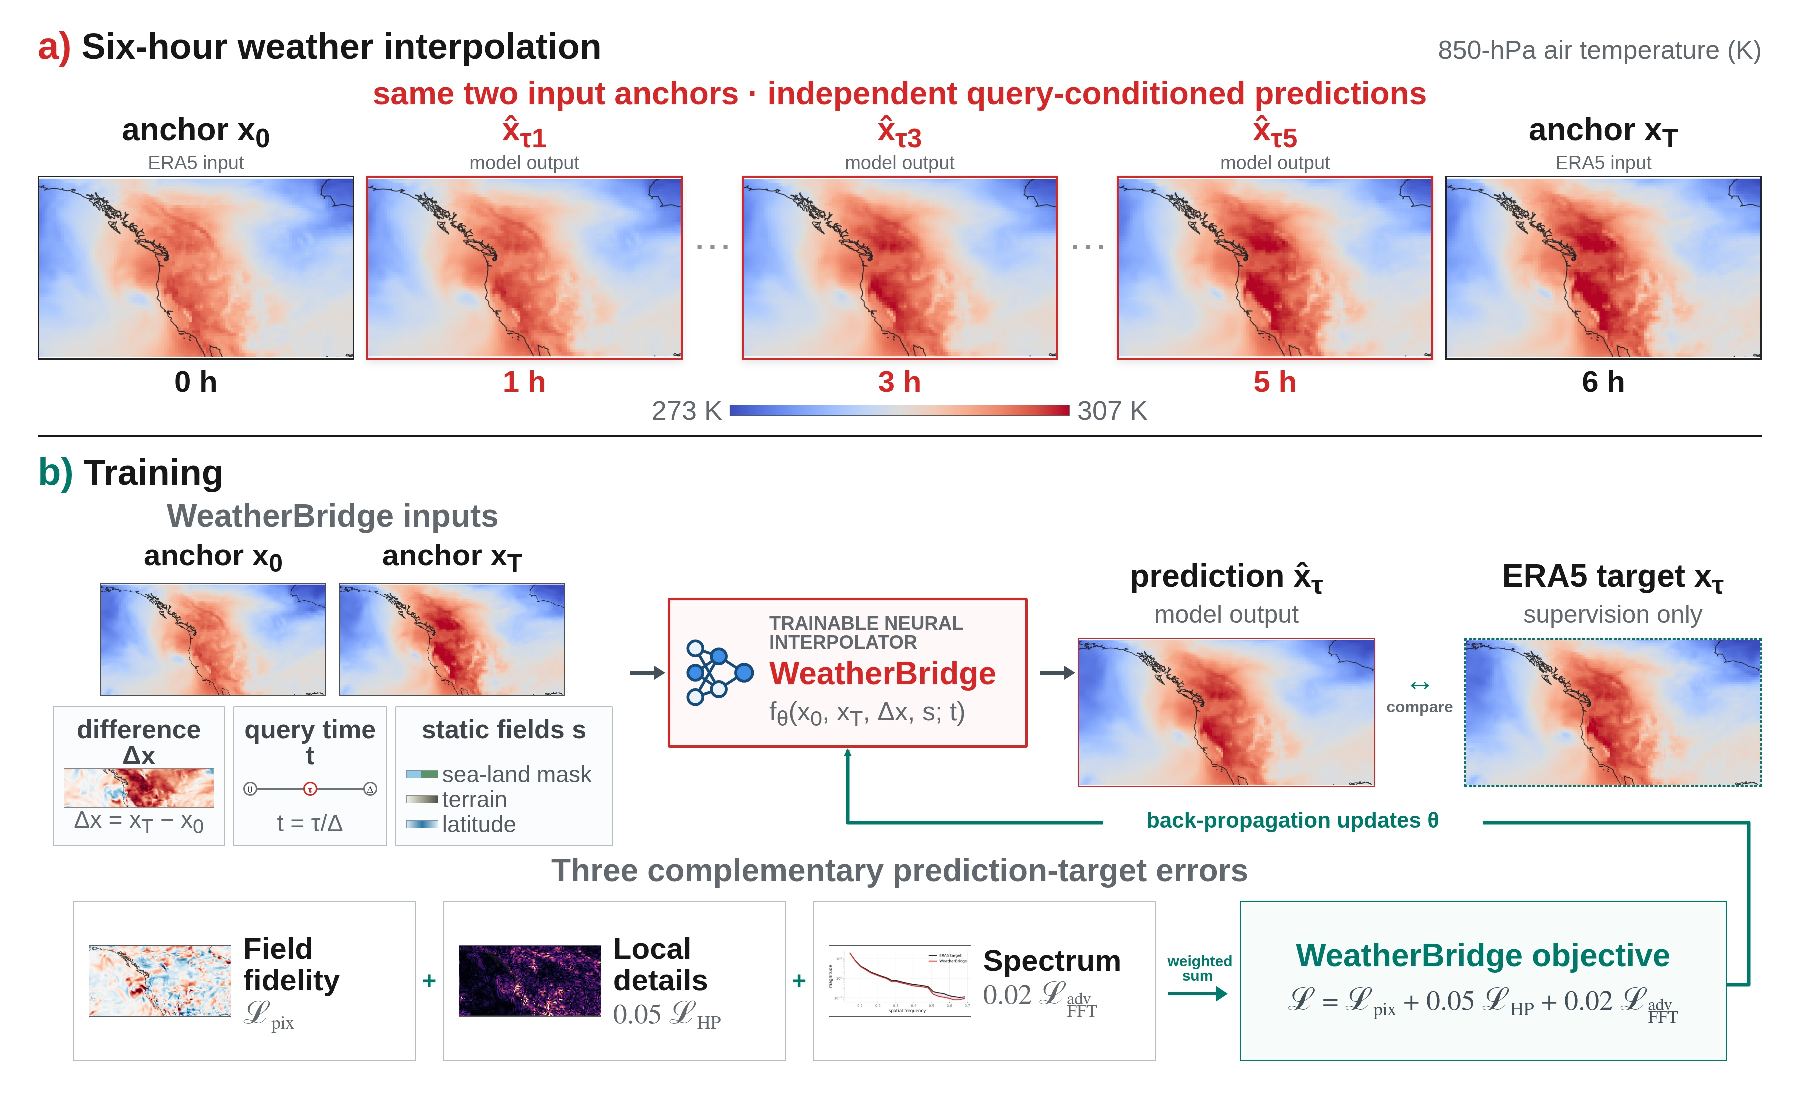
\includegraphics[width=\textwidth]{images/fig_graphical_overview.pdf}
\caption{WeatherBridge interpolation and training workflow. \textbf{a)}
Six-hour reconstruction of 850-hPa air temperature during the Pacific
Northwest heatwave of 28--29 June 2021. The same anchors condition independent
predictions at each query time; ellipses denote the omitted second and fourth
hours. \textbf{b)} Training uses the anchors, their difference, static fields
and $t=\tau/\Delta$. The interior ERA5 state supplies only the pixel,
high-pass and spectral error terms. The green path is active during
back-propagation and absent at inference.}
\label{fig:graphical_overview}
\end{figure}

Weather time interpolation has received less controlled study than weather
forecasting. ModAFNO \cite{leinonen2024modafno} adds $\tau$ conditioning to
an Adaptive Fourier Neural Operator; DYffusion
\cite{cachay2023dyffusion} couples interpolation and forecasting in a
probabilistic sampler. Its diffusion process uses temporal interpolation
in place of the Gaussian noising process of denoising diffusion models
\cite{ho2020ddpm}. Spherical DYffusion applies this framework to global
climate emulation with spherical operators \cite{cachay2024spherical}.
SpateGAN-ERA5 \cite{vandeschrik2024spategan} instead addresses generative
spatial and temporal downscaling of precipitation. Recent task-specific
systems extend the range: HFD-CF \cite{wang2026hfdcf} combines
variable-specific flow with multiresolution warping for four midpoint fields,
MSF-TCMA \cite{gao2025msftcma} combines multiscale wavelet and multi-source
features with a continuous-time manifold on regional unseen-time tests,
while HourGlass \cite{ingstad2026hourglass} reconstructs probabilistic,
temporally coherent trajectories from forecast-system output. Their
variables, resolutions, training sources and query-time protocols differ, so
published scores do not resolve the architectural comparison or behaviour at
longer anchor intervals.
Generative nowcasting models learn future precipitation distributions
\cite{ravuri2021nowcasting,zhang2023nowcastnet}, neural weather models such
as MetNet forecast precipitation directly from observations
\cite{sonderby2020metnet}, and CorrDiff reconstructs
fine spatial structure conditional on coarse atmospheric fields
\cite{mardani2025corrdiff}.

Video-frame interpolation suggests three useful mechanism families. Direct
synthesis avoids an explicit flow field \cite{kalluri2023flavr}; VFIformer and
EMA-VFI aggregate long-range or inter-frame evidence with attention
\cite{shi2022vfiformer,zhang2023emavfi}; and DAIN, RIFE, IFRNet and AMT estimate
motion before fusing transported endpoints
\cite{bao2019dain,huang2022rife,kong2022ifrnet,li2023amt}. Quadratic Video Interpolation
and EQVI add acceleration for non-uniform motion
\cite{xu2019qvi,liu2020eqvi}, while softmax splatting treats collisions during
forward warping \cite{niklaus2020softmax}.
Super SloMo makes intermediate time an explicit input
\cite{jiang2018superslomo}; FILM handles large image motion with multiscale
features \cite{reda2022film}. Diffusion models have also been applied to
frame interpolation \cite{voleti2022mcvd,danier2024ldmvfi}.

Global atmospheric fields change the requirements behind these mechanisms.
Longitude is periodic, grid cells have unequal area, the poles are coordinate
singularities, and 24 variables must remain mutually consistent. Spectral
power can look correct even when a front is displaced, whereas a smoother
field can reduce pointwise error while erasing an informative residual. We
therefore evaluate transport together with spherical scalar and vector
spectra, diagnostic balances and temporal consistency. WeatherBridge adapts
second-order transport to this setting; the quadratic displacement formula
itself follows prior VFI work.

We compare explicit anchor transport with additive encoder--decoder
reconstruction under a common 24-field protocol. The benchmark includes a
time-conditioned SwinV2 \cite{liu2022swinv2}, ModAFNO, S-DYff with Spherical
FNO \cite{bonev2023sfno}, PixelAttn-VFI, the DC-AE-derived WeatherDCAE
\cite{cai2024dcae}, and WeatherBridge. SwinV2 and WeatherDCAE represent direct
residual synthesis, PixelAttn-VFI represents feature-level endpoint
interaction, and WeatherBridge supplies explicit transport. These are
weather-specific implementations inspired by the cited model families rather
than reproductions of image-domain systems. Because their objectives and
update budgets differ, the benchmark measures paper-scale performance rather
than matched-compute efficiency.

Fig.~\ref{fig:tikz_flow} shows how WeatherBridge combines anchor transport
with additive reconstruction. Transport moves existing weather structures
towards the query state; additive branches represent changes in their
amplitude and shape. A learned gate combines transported anchors with
linear interpolation, and a final temperature-column head adjusts
geopotential and mean sea-level pressure.
The study makes three contributions, each tied to a separate experiment:
\begin{enumerate}
\item \textbf{Held-out query-hour benchmark.} Six weather-adapted architectures share a
24-field protocol. A matched WeatherBridge control trained on every interior
hour isolates query withholding from intrinsic hour difficulty. This supports
transfer to sampled unseen queries, not continuous-time generalisation; the
12\,h experiment remains an interval-length ablation.

\item \textbf{WeatherBridge.} A linear residual scaffold is combined with
bidirectional second-order transport, multiscale corrections and spectral
supervision. The model gives the lowest aggregate error at held-out query hours at both
anchor intervals, with field-level exceptions; same-checkpoint lesions test
acceleration, warped-anchor transport and the hydrostatic head.

\item \textbf{Forecast-trajectory transfer.} ERA5-trained models lose their
advantage on IFS HRES anchors. Limited HRES adaptation restores an aggregate
gain over linear interpolation, separating interpolation skill from
anchor-domain mismatch; native data-driven forecast trajectories remain
untested.
\end{enumerate}
\FloatBarrier

\begin{deferredmethodsintro}
\section{Methods}
\label{sec:method}

All learned models receive the same anchor states, static fields and query
time, but differ in how they construct the interior state. We retain the
endpoint chord explicitly so that each network learns transport or curvature
relative to a common linear reference.

\subsection{Problem formulation}

Let $x_0, x_T \in \mathbb{R}^{C \times H \times W}$ denote the two
anchor states with $C{=}24$ channels and $(H, W){=}(360, 720)$. With
$t=\tau/\Delta\in(0,1)$, the additive encoder--decoder baselines use
\begin{equation}
\hat{x}_\tau =
\underbrace{(1-t)x_0+t x_T}_{x_{\mathrm{lin}}}
+\tanh(\alpha)\,v_\theta(x_0,x_T,t,S),
\label{eq:scaffold}
\end{equation}
where $\Delta \in \{6, 12\}\,$h and the static-feature stack $S$ contains the
land-sea mask, normalised surface orography and the pinned cosine-latitude
channel described in Sec.~\ref{sec:setup}. The residual scale is initialised at
$0.10$, is scalar in WeatherDCAE and channelwise in PixelAttn-VFI, and has no
post-activation floor. WeatherBridge uses the distinct transport-and-fusion
path below; its residual gain is also channelwise and initialised at $0.10$.
All three retain $x_{\mathrm{lin}}$ as an explicit fallback.
This separates the known endpoint chord from the temporal curvature and
transported sub-anchor structure that must be learned.

\subsection{Architectures evaluated}

We evaluate the learned architecture families at $0.5^\circ$ resolution
with common anchor states, targets, query hours and scoring code. The main
6\,h comparison uses six training years for every learned model, including
WeatherDCAE-14M. The 12\,h interval-length ablation uses the
common three-year data protocol defined in Sec.~\ref{sec:12h}.
Learning rates, training years and update budgets are listed in
Supplementary Table~\ref{S-tab:protocol_summary}; architecture settings are
in Supplementary Table~\ref{S-tab:hyperparams}.

Linear interpolation is the closed-form, zero-parameter reference and
the fallback state used by the learned synthesis paths.

\paragraph{SwinV2.}
The compact patch-token baseline concatenates the anchors and static fields
into $[x_0,x_T,S]$. A $4\times4$ stride-four convolution produces
256-dimensional tokens. Eight SwinV2 blocks \cite{liu2022swinv2}, arranged as
four windowed/shifted-window pairs, use eight attention heads, a $5\times9$
latitude--longitude window, an MLP expansion ratio of four and stochastic
depth increasing from zero to 0.1. A 128-component sinusoidal encoding of $t$
is projected to featurewise scale and shift after every block. LayerNorm, a
$1\times1$ projection, PixelShuffle and bilinear resizing return a 24-channel
residual, which is multiplied by a learned scalar before addition to
$x_{\mathrm{lin}}$. The model borrows the SwinV2 block family used by FuXi
\cite{chen2023fuxi}, but not FuXi's cascade or full U-Transformer.
The shifted-window hierarchy follows Swin \cite{liu2021swin}; the
time-dependent scale and shift use featurewise conditioning
\cite{perez2018film}.

\paragraph{ModAFNO and S-DYff.}
\emph{ModAFNO}
\cite{leinonen2024modafno,guibas2022afno} uses a compact 36.9\,M
implementation at 6\,h and the 151.7\,M official \texttt{physicsnemo}
configuration at 12\,h; Supplementary Table~\ref{S-tab:hyperparams} records
both.
The Fourier-operator lineage runs from FNO \cite{li2021fno} to AFNO and its
query-conditioned modulation. \emph{S-DYff} is our interpolation-specific
adaptation of DYffusion \cite{cachay2023dyffusion}, using Spherical FNO
\cite{bonev2023sfno} backbones. An interpolator supplies the initial state;
a second network refines it for $K{=}5$ passes at the requested hour. This
fixed-query refiner replaces the original forecaster and its diffusion-time
schedule; it is not the published Spherical DYffusion climate emulator
\cite{cachay2024spherical}.

Neither DYffusion nor ModAFNO was validated here by reproducing the original
paper's scores on its original data with an author checkpoint. Both were
trained for the present field set and query protocol. Using the official
ModAFNO configuration at 12\,h establishes implementation provenance, not
numerical reproduction of the published benchmark.

The original model rows use one checkpoint and one output per input, with
no averaging across checkpoints, random seeds or stochastic draws. ModAFNO
and the four direct/transport models run in evaluation mode without sampling.
S-DYff also runs in evaluation mode, which disables ordinary dropout, but its
custom stochastic-depth operation remains active with drop probability 0.1.
Its row therefore measures a single stochastic reconstruction, not an
ensemble mean. Stochastic depth \cite{huang2016stochastic} and Monte Carlo
dropout \cite{gal2016dropout} are distinct inference mechanisms. Original
DYffusion evaluates ensemble-mean error and probabilistic scores; we do not
reproduce that sampling protocol or report CRPS. The S-DYff ranking concerns
this adaptation, not DYffusion's ensemble skill.
The additional S-DYff-ENS curves average $N=21$ stochastic reconstructions
from the same checkpoint before computing RMSE and ACC. They retain the
same stochastic-depth sampler, with ordinary dropout disabled; no model is
retrained. S-DYff denotes the original $N=1$ result throughout.
To isolate the averaging effect, a separate paired comparison uses nested
prefixes of $N=1,4,16,21$ draws from one sampling stream. Its $N=1$ control
is a fresh draw, not the archived S-DYff result. Seven-day block-bootstrap
intervals quantify evaluation-date variability conditional on that sampling
seed.

\paragraph{PixelAttn-VFI.}
The two endpoints remain separate until the bottleneck. A shared encoder
processes $[x_0,S]$ and $[x_T,S]$ through four scales with 72, 144, 288 and
576 channels; each scale uses two $3\times3$ convolution--GroupNorm--SiLU
blocks, and the final three scales begin with stride-two downsampling. The
deepest endpoint maps are flattened, concatenated and updated by eight-head
self-attention \cite{vaswani2017attention}. Their two token sequences are
then averaged and reshaped. A
128-component time embedding supplies a zero-initialised adaptive gate,
following the conditioning idea in DiT~\cite{peebles2023dit}, at this
bottleneck. Three decoder stages apply a $4\times4$ stride-two transposed
convolution, concatenate the mean endpoint features at the corresponding
scale and apply the same two-convolution block. A zero-initialised head
predicts 24 residual channels with learned channelwise gains. The model tests
feature-level endpoint interaction without a displacement field, correlation
pyramid or warping operator.

\paragraph{WeatherDCAE-14M.}
The direct-synthesis reference encodes $[x_0,x_T,S]$ through three
64/128/256-channel stages with three blocks per stage. The first two stages use
residual convolutions \cite{he2016resnet}; the deepest uses three EfficientViT
blocks \cite{cai2023efficientvit} with
multiscale linear attention, kernel scale five and 32-channel heads.
PixelUnshuffle performs downsampling and a pole-aware projection produces a
256-channel latent. Longitude is padded periodically; samples crossing a pole
are reflected in latitude and shifted by half the longitude span. Eight
latitude rows are replicate-padded before the encoder to make the reported
$0.5^\circ$ checkpoint shape-compatible. The decoder uses two PixelShuffle
stages and pole-aware residual blocks, but no cross-scale encoder--decoder
skips. A final convolution predicts a 24-channel residual scaled by one
learned scalar. This boundary operator is an equirectangular convention, not
a rotationally equivariant spherical convolution.

Supplementary Fig.~\ref{S-fig:reference_architectures} traces these three
comparator implementations from their common inputs to the residual output.

\paragraph{WeatherBridge.}
The proposed transport-aware model uses $t=\tau/\Delta$ as query time
normalised by the anchor interval. Its input
is $[x_0,x_T,x_T-x_0,S]$, where $S$ contains land--sea mask, orography and the
pinned cosine-latitude feature. A sinusoidal embedding followed by a
256-dimensional multilayer perceptron conditions both the AdaLN-Zero
bottleneck and the three decoder skip connections. The cross-scale
encoder--decoder connections
follow the U-Net pattern \cite{ronneberger2015unet}. The shared block
$B(c_{\rm in},c_{\rm out},s)$ applies a $3\times3$ convolution with stride
$s$ and the checkpoint's circular padding in both tensor dimensions,
followed by GroupNorm \cite{wu2018groupnorm} and SiLU; a second $3\times3$
convolution uses stride
one. The longitude wrap is physical, whereas the resulting adjacency between
the northernmost and southernmost rows is an implementation artefact. For
decoder level $i$, $u$ is the upsampled decoder feature and
$E_i$ is the encoder feature at the same resolution. The block labelled
``Skip connection'' in Fig.~\ref{fig:tikz_flow} computes
$u+\tanh(g_i(t))\odot P_{3\times3}[u,E_i]$ before applying $B$. Thus the short
label refers to a query-time-gated skip rather than a plain U-Net
concatenation.
Here brackets denote channel concatenation, $P_{3\times3}$ is a learned
convolution followed by GroupNorm and SiLU, and $g_i(t)$ is a channelwise gate obtained
by a SiLU--linear projection of the time embedding. The symbol $\odot$
denotes elementwise multiplication.

\emph{Motion and anchor blending.}
The decoder produces $h_t^{(0)}$ at $360\times720$ and $h_t^{(1)}$ at
$180\times360$, with 72 and 144 feature channels, respectively.
$\Phi_{\rm mot}$ and $\Phi_\alpha$ denote two separate learned
$3\times3$ convolutions applied to $h_t^{(0)}$.
The motion head has eight outputs, arranged as four two-component maps:
$(F_0,F_T,A_0,A_T)=8\tanh(\Phi_{\rm mot}(h_t^{(0)}))$.
$F_0,F_T$ are first-order displacement coefficients and $A_0,A_T$
are second-order coefficients, all in grid-pixel units for normalised
time $t$. They are shared across weather channels and are not estimates
of physical wind or material acceleration.
The blend head has 24 outputs and gives
$\alpha_t=\sigma(\Phi_\alpha(h_t^{(0)})+1-2t)$, where $\sigma$ is the
logistic sigmoid. Each channel and grid point therefore has its own weight
for the two warped anchors. The offset $1-2t$ favours the nearer anchor
before learning modifies the blend.

\emph{Additive reconstruction.}
Two further $3\times3$ convolutions map $h_t^{(0)}$ and $h_t^{(1)}$ to
24-channel fields $\Delta_t^{\mathrm{fine}}$ and
$\Delta_t^{\mathrm{coarse}}$. The operator $\operatorname{up}$ bilinearly
resizes the coarse field to $360\times720$. The fine branch can change
local amplitudes and shapes that displacement alone cannot reconstruct;
the coarse branch predicts corrections with a wider spatial context.
Both outputs are in normalised weather-field units, not displacement units.
The third contribution, $G_t^{\mathrm{SFNO}}$, comes from a spherical
Fourier neural operator branch \cite{bonev2023sfno} applied to $h_t^{(0)}$.
A $1\times1$ projection reduces its width to 20 channels; learned complex
weights mix channels over the retained spherical-harmonic modes
($\ell,m<20$). The inverse transform is added to the projected features,
followed by GELU and a $1\times1$ projection to 24 fields. This gives
the residual global spatial context. Only its spectral operation is
low-wavenumber: the local path and nonlinearity mean that the output
need not be strictly band-limited. All three output projections are
zero-initialised. Their sum is $\Delta_t$; these are architectural
corrections, not additional loss terms.

The two anchors are warped and combined with these corrections as follows:
\begin{equation}
\begin{aligned}
d_0(t) &= F_0(t)t+\tfrac12 A_0(t)t^2,\qquad
d_T(t)=F_T(t)(1-t)+\tfrac12 A_T(t)(1-t)^2,\\
W_0 &= \mathcal W(x_0,d_0),\qquad W_T=\mathcal W(x_T,d_T),\\
x_{\mathrm{lin}}&=(1-t)x_0+t x_T,\\
x_{\mathrm{tr}} &= \alpha_t\odot W_0
 +(1-\alpha_t)\odot W_T,\\
\Delta_t &= \Delta_t^{\mathrm{fine}}
 +\operatorname{up}(\Delta_t^{\mathrm{coarse}})+G_t^{\mathrm{SFNO}},\\
x_{\mathrm{mix}} &= \beta\odot x_{\mathrm{tr}}
 +(1-\beta)\odot x_{\mathrm{lin}},\\
x_{\mathrm{pre}} &= x_{\mathrm{mix}}+\tanh(\gamma)\odot\Delta_t,\\
\widehat{x}_t &= x_{\mathrm{pre}}+
\mathcal I_{Z,\mathrm{MSLP}}\,H_T(x_{\mathrm{pre}}),
\end{aligned}
\label{eq:flow_scaffold}
\end{equation}
where $\mathcal{W}$ is differentiable bilinear warping~\cite{jaderberg2015stn} on the
lat--lon grid, $\beta=\sigma(b)$ is a learned per-channel gate between
transport and the linear scaffold, $\gamma$ is the learned per-channel
residual gain. Unlike the spatially varying $\alpha_t$, $\beta$ and
$\gamma$ are learned vectors with one value per weather channel.
$x_{\mathrm{tr}}$ is the transported-anchor blend,
$x_{\mathrm{mix}}$ also includes the unwarped linear estimate, and
$x_{\mathrm{pre}}$ adds the scaled residual.

\emph{Temperature-column correction.}
$H_T$ is a zero-initialised $1\times1$ convolution that reads the four
predicted temperature channels of $x_{\mathrm{pre}}$ at
1000, 925, 850 and 700\,hPa and outputs five corrections.
$\mathcal I_{Z,\mathrm{MSLP}}$ inserts them into geopotential at those
levels and MSLP, leaving the other 19 channels unchanged. In
Fig.~\ref{fig:tikz_flow}, $\Delta_{\mathrm{hydro}}$ denotes this
24-channel insertion, including its zero entries.
The head is motivated by the relation between temperature and geopotential
thickness. It learns a local column adjustment; it does not integrate the
hydrostatic equation or enforce an exact balance.
The linear scaffold remains an explicit fallback while the model
separately represents displacement, additive field changes and
temperature--mass-field coupling.
The trunk is a latitude--longitude convolutional network. We account for spherical geometry in
evaluation through strip-area weights and spherical-harmonic diagnostics.
Within the network, the spectral operation in the SFNO branch uses a
spherical-harmonic basis.
The convolutional encoder processes the anchors and static fields without
time modulation. Conditioning enters at the AdaLN-Zero bottleneck and the
decoder skip gates, making $F_i(t)$ and $A_i(t)$ query-specific coefficients.
Each query receives its own second-order
displacement; these coefficients describe separate query states rather than a
parcel trajectory through all interior times.

WeatherDCAE-14M and WeatherBridge differ in both backbone and synthesis path;
their comparison is architectural rather than a single-component ablation.

\paragraph{Retrained architecture variants.}
Refine uses shared field controls, a 16-token area-weighted latent transformer
and two decoder blocks per level, and omits the temperature-conditioned
mass-field head. It has 13.7 million parameters and is trained from scratch.
Several mechanisms change together, so this comparison does not isolate
one component. Detail adds an anchor-detail bypass to the WeatherBridge
trunk. The same flows and blend gate transport the finest pole-aware local
multiband component of each anchor. A $t$-conditioned gain reinjects the
difference between this transported detail and the model's own detail.
The gain is initialised at zero, bounded to $\pm0.5$ and multiplied by
$4t(1-t)$, where $t=\tau/\Delta$; Detail initially reproduces its parent.
Supplementary Table~\ref{S-tab:architecture-ablation} reports the retrained
variants. The separate same-checkpoint lesions disable acceleration,
warped-anchor transport or the hydrostatic head without retraining.

\end{deferredmethodsintro}

\begin{figure*}[!t]
\centering
\resizebox{\textwidth}{!}{%
\def\archtitle#1{{\sffamily\bfseries\fontsize{7.4}{7.8}\selectfont #1}}
\def\archsmalltitle#1{{\sffamily\bfseries\fontsize{6.8}{7.2}\selectfont #1}}

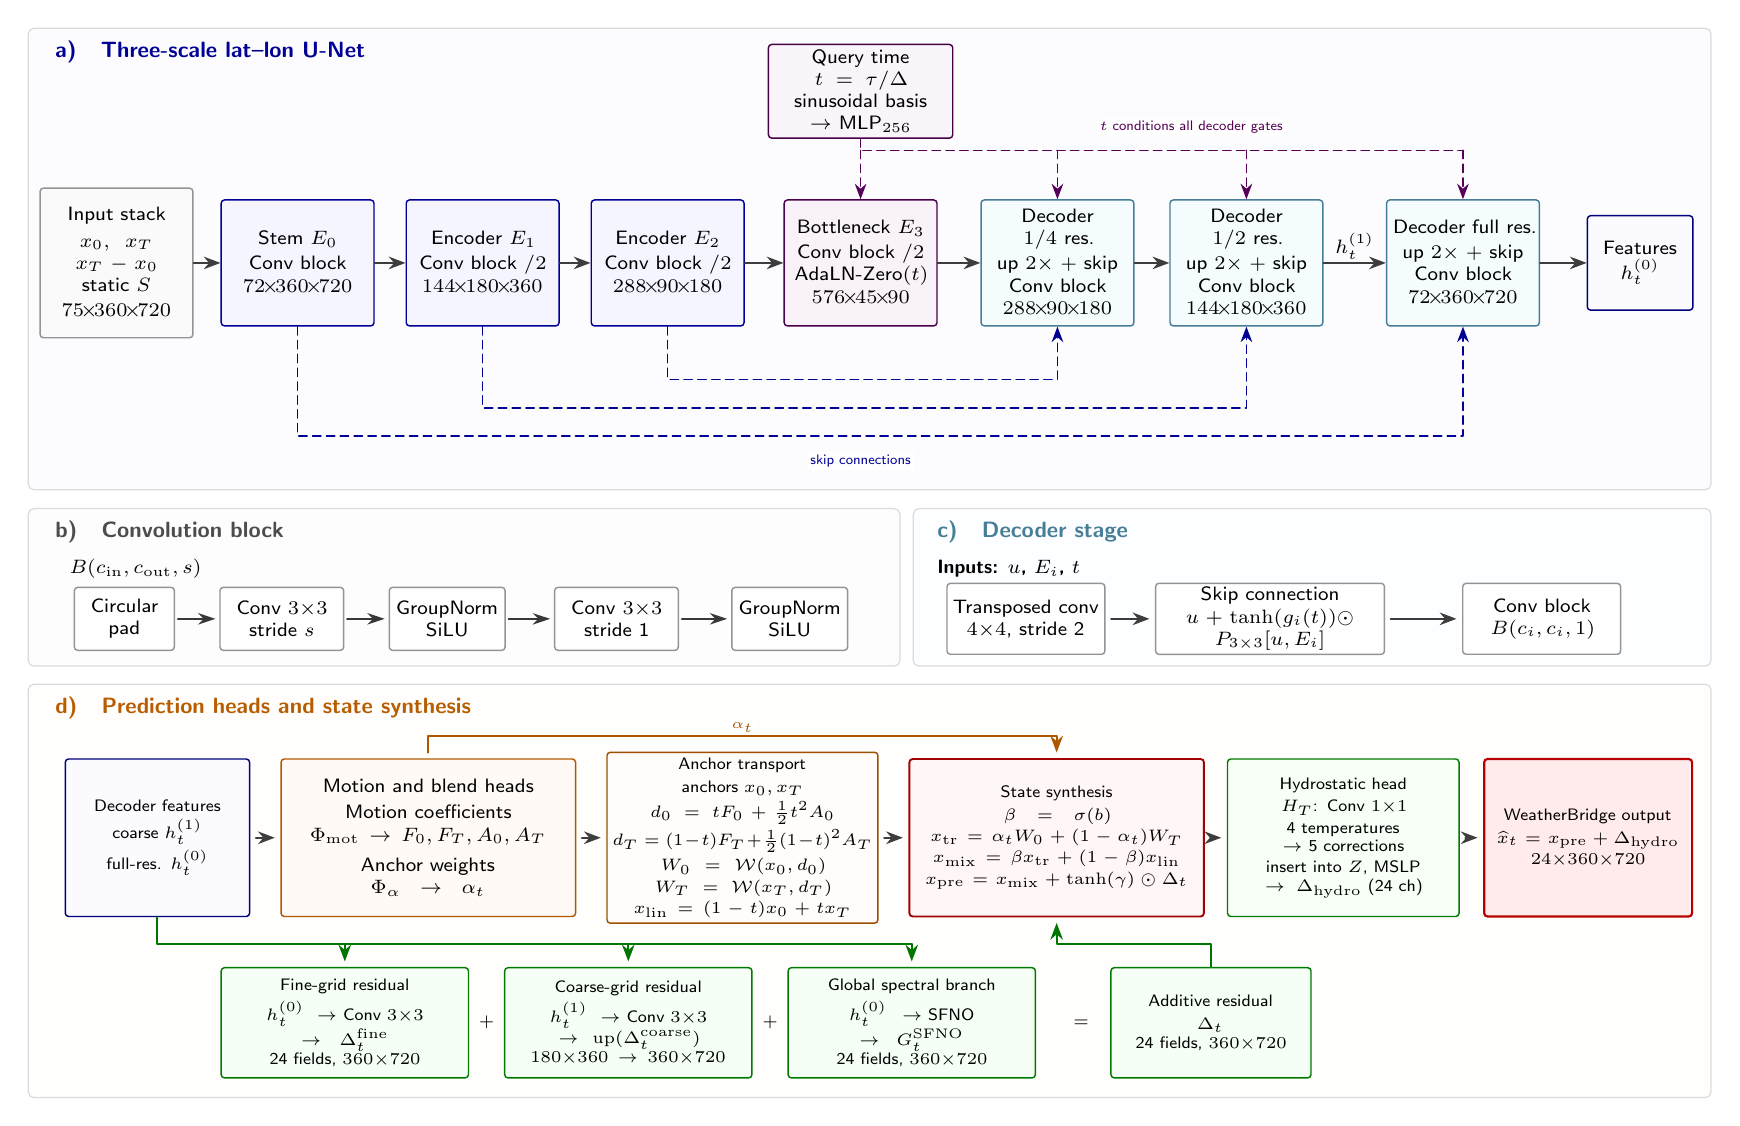
\begin{tikzpicture}[
  x=1cm,
  y=1cm,
  >={Stealth[length=1.8mm, width=1.2mm]},
  font=\sffamily\scriptsize,
  box/.style={
    rectangle,
    draw=black!42,
    rounded corners=1.2pt,
    align=center,
    inner xsep=2.0pt,
    inner ysep=2.0pt,
    line width=0.52pt
  },
  stage/.style={
    box,
    fill=blue!4,
    draw=blue!58!black,
    text width=18mm,
    minimum height=16mm
  },
  decoder/.style={
    stage,
    fill=cyan!4,
    draw=cyan!55!black
  },
  bottleneck/.style={
    box,
    fill=violet!5,
    draw=violet!58!black,
    text width=18mm,
    minimum height=16mm
  },
  input/.style={
    box,
    fill=black!2,
    text width=18mm,
    minimum height=19mm
  },
  feature/.style={
    box,
    fill=blue!2,
    draw=blue!48!black,
    text width=16mm,
    minimum height=12mm
  },
  time/.style={
    box,
    fill=violet!4,
    draw=violet!55!black,
    text width=22mm,
    minimum height=7mm
  },
  operation/.style={
    box,
    fill=white,
    text width=16mm,
    minimum height=9mm,
    inner xsep=1.5pt,
    inner ysep=1.5pt
  },
  operation wide/.style={
    operation,
    text width=19mm
  },
  operation compact/.style={
    operation,
    text width=14mm,
    minimum height=8mm,
    inner xsep=1pt
  },
  operation compact wide/.style={
    operation compact,
    text width=17mm
  },
  interface/.style={
    box,
    fill=black!2,
    text width=14mm,
    minimum height=17mm
  },
  heads/.style={
    box,
    fill=orange!4,
    draw=orange!70!black,
    text width=21mm,
    minimum height=20mm
  },
  warp/.style={
    box,
    fill=orange!2,
    draw=orange!62!black,
    text width=21mm,
    minimum height=20mm
  },
  correction/.style={
    box,
    fill=green!4,
    draw=green!48!black,
    text width=44mm,
    minimum height=9mm
  },
  synthesis/.style={
    box,
    fill=red!3,
    draw=red!64!black,
    text width=25mm,
    minimum height=21mm,
    line width=0.68pt
  },
  physics/.style={
    box,
    fill=green!3,
    draw=green!48!black,
    text width=17mm,
    minimum height=16mm
  },
  output/.style={
    box,
    fill=red!8,
    draw=red!72!black,
    text width=22mm,
    minimum height=15mm,
    line width=0.78pt
  },
  flow/.style={
    -Stealth,
    draw=black!76,
    line width=0.68pt,
    line cap=round,
    line join=round
  },
  blockflow/.style={
    -{Stealth[length=2.2mm, width=1.45mm]},
    draw=black!78,
    line width=0.72pt,
    line cap=round,
    shorten <=1.0pt,
    shorten >=1.4pt
  },
  skip/.style={
    -Stealth,
    draw=blue!58!black,
    densely dashed,
    line width=0.58pt,
    line cap=round,
    line join=round
  },
  condition/.style={
    -Stealth,
    draw=violet!68!black,
    densely dashed,
    line width=0.58pt,
    line cap=round,
    line join=round
  },
  panel/.style={
    font=\sffamily\bfseries\footnotesize,
    anchor=west
  },
  edge label/.style={
    font=\sffamily\tiny,
    fill=white,
    inner sep=1pt,
    text=black!58
  }
]

% The large top panel exposes every resolution of the shared U-Net.
\begin{scope}[on background layer]
  \fill[blue!1.25, rounded corners=2pt] (-0.12,4.42)
    rectangle (21.25,10.28);
  \draw[black!14, rounded corners=2pt, line width=0.45pt] (-0.12,4.42)
    rectangle (21.25,10.28);

  \fill[black!0.8, rounded corners=2pt] (-0.12,2.18)
    rectangle (10.95,4.18);
  \draw[black!14, rounded corners=2pt, line width=0.45pt] (-0.12,2.18)
    rectangle (10.95,4.18);

  \fill[cyan!1.2, rounded corners=2pt] (11.12,2.18)
    rectangle (21.25,4.18);
  \draw[black!14, rounded corners=2pt, line width=0.45pt] (11.12,2.18)
    rectangle (21.25,4.18);

  \fill[orange!0.9, rounded corners=2pt] (-0.12,-3.30)
    rectangle (21.25,1.95);
  \draw[black!14, rounded corners=2pt, line width=0.45pt] (-0.12,-3.30)
    rectangle (21.25,1.95);
\end{scope}

\node[panel, text=blue!58!black] at (0.10,9.98)
  {\textbf{a)}\quad Three-scale lat--lon U-Net};
\node[panel, text=black!70] at (0.10,3.88)
  {\textbf{b)}\quad Convolution block};
\node[panel, text=cyan!55!black] at (11.30,3.88)
  {\textbf{c)}\quad Decoder stage};
\node[panel, text=orange!72!black] at (0.10,1.65)
  {\textbf{d)}\quad Prediction heads and state synthesis};

% a) End-to-end encoder-decoder backbone.
\node[input] (inputs) at (1.00,7.30)
  {\archtitle{Input stack}\\[1.5pt]
   $x_0,\;x_T$\\
   $x_T-x_0$\\
   static $S$\\[1pt]
   $75\!{\times}\!360\!{\times}\!720$};

\node[stage] (e0) at (3.30,7.30)
  {\archtitle{Stem $E_0$}\\[1pt]
   Conv block\\
   $72\!{\times}\!360\!{\times}\!720$};
\node[stage] (e1) at (5.65,7.30)
  {\archtitle{Encoder $E_1$}\\[1pt]
   Conv block $/2$\\
   $144\!{\times}\!180\!{\times}\!360$};
\node[stage] (e2) at (8.00,7.30)
  {\archtitle{Encoder $E_2$}\\[1pt]
   Conv block $/2$\\
   $288\!{\times}\!90\!{\times}\!180$};
\node[bottleneck] (e3) at (10.45,7.30)
  {\archtitle{Bottleneck $E_3$}\\[1pt]
   Conv block $/2$\\
   AdaLN-Zero$(t)$\\
   $576\!{\times}\!45\!{\times}\!90$};

\node[decoder] (d2) at (12.95,7.30)
  {\archtitle{Decoder $1/4$ res.}\\[1pt]
   up $2{\times}$ + skip\\
   Conv block\\
   $288\!{\times}\!90\!{\times}\!180$};
\node[decoder] (d1) at (15.35,7.30)
  {\archtitle{Decoder $1/2$ res.}\\[1pt]
   up $2{\times}$ + skip\\
   Conv block\\
   $144\!{\times}\!180\!{\times}\!360$};
\node[decoder] (d0) at (18.10,7.30)
  {\archtitle{Decoder full res.}\\[1pt]
   up $2{\times}$ + skip\\
   Conv block\\
   $72\!{\times}\!360\!{\times}\!720$};
\node[feature, text width=12mm] (features) at (20.35,7.30)
  {\archtitle{Features}\\[1pt]$h_t^{(0)}$};

\draw[flow] (inputs.east) -- (e0.west);
\draw[flow] (e0.east) -- (e1.west);
\draw[flow] (e1.east) -- (e2.west);
\draw[flow] (e2.east) -- (e3.west);
\draw[flow] (e3.east) -- (d2.west);
\draw[flow] (d2.east) -- (d1.west);
\draw[flow] (d1.east) -- node[above,inner sep=1pt] {$h_t^{(1)}$} (d0.west);
\draw[flow] (d0.east) -- (features.west);

\node[time] (time) at (10.45,9.48)
  {\archtitle{Query time}\quad $t=\tau/\Delta$\qquad
   sinusoidal basis $\rightarrow$ MLP$_{256}$};
% A common conditioning bus keeps all decoder arrows vertical and separate.
\draw[condition, -] (time.south) -- (10.45,8.73) -- (18.10,8.73);
\draw[condition] (10.45,8.73) -- (e3.north);
\draw[condition] (12.95,8.73) -- (d2.north);
\draw[condition] (15.35,8.73) -- (d1.north);
\draw[condition] (18.10,8.73) -- (d0.north);
\node[edge label, text=violet!65!black] at (14.65,9.02)
  {$t$ conditions all decoder gates};

% Nested skip routes are deliberately separated vertically.
\draw[skip] (e2.south) -- (8.00,5.82) -- (12.95,5.82) -- (d2.south);
\draw[skip] (e1.south) -- (5.65,5.46) -- (15.35,5.46) -- (d1.south);
\draw[skip] (e0.south) -- (3.30,5.10) -- (18.10,5.10) -- (d0.south);
\node[edge label, text=blue!58!black] at (10.45,4.78)
  {skip connections};

% b) Reused convolution block.
\node[anchor=west, font=\sffamily\bfseries\scriptsize] at (0.28,3.42)
  {$B(c_{\rm in},c_{\rm out},s)$};
\node[operation compact, text width=12mm] (pad1) at (1.10,2.78)
  {\archtitle{Circular pad}};
\node[operation compact wide, text width=15mm] (conv1) at (3.10,2.78)
  {\archtitle{Conv $3{\times}3$}\\stride $s$};
\node[operation compact, text width=14mm] (norm1) at (5.20,2.78)
  {\archtitle{GroupNorm}\\SiLU};
\node[operation compact wide, text width=15mm] (conv2) at (7.35,2.78)
  {\archtitle{Conv $3{\times}3$}\\stride 1};
\node[operation compact, text width=14mm] (norm2) at (9.55,2.78)
  {\archtitle{GroupNorm}\\SiLU};
\draw[blockflow] (pad1.east) -- (conv1.west);
\draw[blockflow] (conv1.east) -- (norm1.west);
\draw[blockflow] (norm1.east) -- (conv2.west);
\draw[blockflow] (conv2.east) -- (norm2.west);

% c) Reused decoder stage.
\node[anchor=west, font=\sffamily\bfseries\scriptsize] at (11.30,3.42)
  {Inputs: $u$, $E_i$, $t$};
\node[operation wide] (up) at (12.55,2.78)
  {\archtitle{Transposed conv}\\$4{\times}4$, stride 2};
\node[operation, text width=28mm] (gate) at (15.65,2.78)
  {\archtitle{Skip connection}\\
   $u+\tanh(g_i(t))\odot$
   $P_{3{\times}3}[u,E_i]$};
\node[operation wide] (block) at (19.10,2.78)
  {\archtitle{Conv block}\\$B(c_i,c_i,1)$};
\draw[flow, shorten <=2pt, shorten >=2pt] (up.east) -- (gate.west);
\draw[flow, shorten <=2pt, shorten >=2pt] (gate.east) -- (block.west);

% d) Decoder features parameterise transport and additive correction.
\begin{scope}[font=\sffamily\fontsize{6.0}{6.7}\selectfont]
% Node widths follow their longest formula. Equal edge gaps keep every
% main-path arrow horizontal despite the different aspect ratios.
\node[feature, text width=22mm, minimum height=20mm] (head-input) at (1.52,0.00)
  {\archsmalltitle{Decoder features}\\[1.5pt]
   coarse $h_t^{(1)}$\\[1pt]
   full-res. $h_t^{(0)}$};

\node[heads, text width=36mm, minimum height=20mm,
  font=\sffamily\fontsize{7.2}{8.0}\selectfont] (heads) at (4.96,0.00)
  {\archsmalltitle{Motion and blend heads}\\[1.5pt]
   Motion coefficients\\
   $\Phi_{\rm mot}\rightarrow F_0,F_T,A_0,A_T$\\[3pt]
   Anchor weights\\
   $\Phi_\alpha\rightarrow\alpha_t$};

\node[warp, text width=33mm, minimum height=20mm] (operators) at (8.95,0.00)
  {\archsmalltitle{Anchor transport}\\[1.5pt]
   anchors $x_0,x_T$\\[1pt]
   $d_0=tF_0+\tfrac12t^2A_0$\\[1pt]
   $d_T=(1-t)F_T+\tfrac12(1-t)^2A_T$\\[1pt]
   $W_0=\mathcal W(x_0,d_0)$\\[1pt]
   $W_T=\mathcal W(x_T,d_T)$\\[1pt]
   $x_{\rm lin}=(1-t)x_0+t x_T$};

\node[synthesis, text width=36mm, minimum height=20mm] (synthesis) at (12.94,0.00)
  {\archsmalltitle{State synthesis}\\[1.5pt]
   $\beta=\sigma(b)$\\[1pt]
   $x_{\rm tr}=\alpha_t W_0+(1-\alpha_t)W_T$\\[1pt]
   $x_{\rm mix}=\beta x_{\rm tr}+(1-\beta)x_{\rm lin}$\\[1pt]
   $x_{\rm pre}=x_{\rm mix}+\tanh(\gamma)\odot\Delta_t$};

\node[physics, text width=28mm, minimum height=20mm] (hydro) at (16.58,0.00)
  {\archsmalltitle{Hydrostatic head}\\[1.5pt]
   $H_T$: Conv $1{\times}1$\\[1pt]
   4 temperatures $\rightarrow$ 5 corrections\\[1pt]
   insert into $Z$, MSLP\\
   $\rightarrow\Delta_{\rm hydro}$ (24 ch)};

\node[output, text width=25mm, minimum height=20mm] (output) at (19.69,0.00)
  {\archsmalltitle{WeatherBridge output}\\[1.5pt]
   $\widehat{x}_t=x_{\rm pre}+\Delta_{\rm hydro}$\\[1pt]
   $24{\times}360{\times}720$};

\node[correction, text width=30mm, minimum height=14mm] (fine) at (3.90,-2.35)
  {\archsmalltitle{Fine-grid residual}\\[1.5pt]
   $h_t^{(0)}\rightarrow$ Conv $3{\times}3$\\
   $\rightarrow\Delta_t^{\rm fine}$\\
   24 fields, $360{\times}720$};
\node[correction, text width=30mm, minimum height=14mm] (coarse) at (7.50,-2.35)
  {\archsmalltitle{Coarse-grid residual}\\[1.5pt]
   $h_t^{(1)}\rightarrow$ Conv $3{\times}3$\\
   $\rightarrow\operatorname{up}(\Delta_t^{\rm coarse})$\\
   $180{\times}360\rightarrow360{\times}720$};
\node[correction, text width=30mm, minimum height=14mm] (global) at (11.10,-2.35)
  {\archsmalltitle{Global spectral branch}\\[1.5pt]
   $h_t^{(0)}\rightarrow$ SFNO\\
   $\rightarrow G_t^{\rm SFNO}$\\
   24 fields, $360{\times}720$};
\node at (5.70,-2.35) {$+$};
\node at (9.30,-2.35) {$+$};
\node at (13.25,-2.35) {$=$};
\node[correction, text width=24mm, minimum height=14mm] (correction) at (14.90,-2.35)
  {\archsmalltitle{Additive residual}\\[1.5pt]
   $\Delta_t$\\
   24 fields, $360{\times}720$};

\draw[flow, shorten <=2pt, shorten >=2pt] (head-input.east) -- (heads.west);
\draw[flow, shorten <=2pt, shorten >=2pt] (heads.east) -- (operators.west);
\draw[flow, shorten <=2pt, shorten >=2pt] (operators.east) -- (synthesis.west);
\draw[flow, shorten <=2pt, shorten >=2pt] (synthesis.east) -- (hydro.west);
\draw[flow, shorten <=2pt, shorten >=2pt] (hydro.east) -- (output.west);
\draw[flow, -, draw=green!46!black]
  (head-input.south) -- (1.52,-1.35) -- (11.10,-1.35);
\foreach \name/\x in {fine/3.90,coarse/7.50,global/11.10}
  \draw[flow, draw=green!46!black, shorten >=2pt]
    (\x,-1.35) -- (\name.north);
\draw[flow, draw=green!46!black, shorten >=2pt]
  (correction.north) -- (14.90,-1.35) -| (synthesis.south);

% Alpha bypasses the geometric warp but remains derived from the same
% full-resolution decoder feature.
\draw[flow, draw=orange!68!black, shorten <=2pt, shorten >=2pt]
  (heads.north) -- ++(0,0.28) -|
  node[edge label, near start, above, text=orange!65!black] {$\alpha_t$}
  (synthesis.north);
\end{scope}

\end{tikzpicture}
%
}
\caption{End-to-end WeatherBridge architecture. \textbf{a)} A
query-conditioned encoder--decoder maps the 75-channel input stack to
multiscale features. \textbf{b)} The convolution block used at each scale.
\textbf{c)} A decoder stage with its query-time-gated skip connection.
\textbf{d)} Full- and coarse-resolution features parameterise
second-order anchor transport and additive reconstruction.
$\Phi_{\rm mot}$ and $\Phi_\alpha$ are learned $3\times3$ convolutions
with eight and 24 output channels, respectively, both applied to
$h_t^{(0)}$. Their outputs give
$(F_0,F_T,A_0,A_T)=8\tanh(\Phi_{\rm mot}(h_t^{(0)}))$ and
$\alpha_t=\sigma(\Phi_\alpha(h_t^{(0)})+1-2t)$.
$F_0,F_T$ and $A_0,A_T$ are first- and second-order
displacement coefficients; $\mathcal W$ resamples an anchor at the
predicted displacement, giving $W_0,W_T$.
$\alpha_t$ blends the warped anchors, $\beta$ mixes that estimate with
linear interpolation, and $\tanh(\gamma)$ scales the additive residual.
The lower branches produce fine-grid, upsampled coarse-grid and global
SFNO (spherical Fourier neural operator) corrections whose sum is
$\Delta_t$; $\operatorname{up}$ is bilinear resizing.
$H_T$ maps the four predicted temperature fields to corrections of
geopotential and MSLP; $\Delta_{\rm hydro}$ is zero in all other channels.
Here $t=\tau/\Delta$, $\sigma$ is the sigmoid and $\odot$ denotes
elementwise multiplication. Methods defines each operation.}
\label{fig:tikz_flow}
\end{figure*}

\begin{deferredmethodsrest}


\subsection{Training objective}
\label{sec:training_objective}

The 14M-scale models minimise latitude-weighted pixel $\ell_1$ error,
\[
\begin{aligned}
\mathcal{L}_{\mathrm{pix}}
&= \frac{1}{BCHW}\sum_{b,c,i,j}
w_i\left|\hat{x}_{bcij}-x_{bcij}\right|,\\
w_i &=\frac{H\cos(\widetilde\phi_i)}
{\sum_{k=1}^{H}\cos(\widetilde\phi_k)}.
\end{aligned}
\]
Here $\widetilde\phi_i$ denotes the legacy symmetric training rows
$89.75^\circ,\ldots,-89.75^\circ$. Thus $\sum_i w_i=H$, and the displayed
normalisation is exactly the tensor reduction implemented by the training
code. The evaluated WeatherBridge run uses unit channel and
query-time weights. This training convention records how the checkpoint was
fitted. All reported evaluation reductions use the block-average coordinates
in Sec.~\ref{sec:setup}. The internal SFNO
branch likewise uses the checkpointed
\href{https://github.com/NVIDIA/torch-harmonics}{\texttt{torch-harmonics}}
equiangular operator \cite{bonev2023sfno} on the stored tensor rows; it is a learned low-mode
feature operator and is distinct from the double-precision diagnostic SHT.
WeatherBridge adds two explicitly separated spectral terms:
\[
\mathcal L_{\mathrm{WeatherBridge}}
 =\mathcal L_{\mathrm{pix}}+0.05\mathcal L_{\mathrm{HP}}
   +0.02\mathcal L_{\mathrm{FFT}}^{\mathrm{adv}}.
\]
Here $\mathcal L_{\mathrm{HP}}$ is a phase-sensitive $3\times3$ local
high-pass $\ell_1$ loss with periodic-longitude and replicated-latitude
padding. $\mathcal L_{\mathrm{FFT}}^{\mathrm{adv}}$
compares magnitudes of the planar fast Fourier transform (FFT) for the
advected-channel mask. The training objective targets planar local detail and
FFT amplitude, whereas the spherical-harmonic evaluation band
$\ell\in[80,180]$ is assessed independently. The
spherical-harmonic-transform (SHT) diagnostic is computed independently after
training. All 24 channels are scored; the FFT term is restricted to the
declared advected-channel mask.
WeatherDCAE-14M and PixelAttn-VFI use $\mathcal L_{\mathrm{pix}}$ alone.
These 14M-scale runs use AdamW \cite{loshchilov2019adamw} with default moment
coefficients, weight decay
$10^{-4}$, a 500-update linear warm-up followed by cosine decay, and
gradient clipping at $\|g\|_2=1.0$.

SwinV2, ModAFNO, and S-DYff use a common forecasting-style baseline recipe.
Their objective combines three terms:
$\mathcal{L} = \mathcal{L}_{\text{recon}}
+ \lambda_{\text{anc}} \mathcal{L}_{\text{anchor}}
+ \lambda_{\text{unit}} \mathcal{L}_{\text{unit}}$,
where $\mathcal{L}_{\text{recon}}$ is a lat-weighted pixel-wise
\emph{smooth-$\ell_1$} (Huber) loss with $\beta{=}0.02$ and Aurora-style
channel weights \cite{bodnar2024aurora}. At 1000/925/850/700\,hPa these
weights are T: 1/1/1/1, U and V: 0.5/0.7/0.9/1.2,
Q: 1.5/1.3/1.0/0.6, and Z: 1.0/0.8/0.5/0.3; the surface weights are
3.0/0.77/0.66/1.5 for T2m/U10/V10/MSLP. Smooth-$\ell_1$ is quadratic for
$|r|<\beta$ and linear in the tails.
$\mathcal{L}_{\text{anchor}}$ penalises drift at $\tau{=}0, \Delta$
($\lambda_{\text{anc}}{=}0.5$, applied every four mini-batches).
The residual branch predicts a correction $v_\theta$ to the linear
interpolation $x_{\mathrm{lin}}$. In SwinV2 and ModAFNO, the principal
reconstruction loss scores $x_{\mathrm{lin}}+g\odot v_\theta$, where $g$ is
the learned residual gain. Auxiliary unit-gain reconstruction evaluates
the same correction with unit residual gain:
\[
\mathcal{L}_{\text{unit}}
 =\mathcal{L}_{\text{recon}}(x_{\mathrm{lin}}+v_\theta,x_\tau),
\qquad \lambda_{\text{unit}}=1.0.
\]
It directly supervises the unscaled correction, even when $g$ is small.
For S-DYff, $v_\theta$ is the interpolator output before gain scaling,
whereas the principal reconstruction loss scores the refined prediction.
The forward pass separately preserves the sign of the learned gain and
clamps its magnitude to at least 0.05.
WeatherBridge also uses a linear interpolation and a residual branch, but
trains that branch through the losses on its final output listed above;
it does not use this auxiliary unit-gain reconstruction loss. Neither
WeatherDCAE-14M nor PixelAttn-VFI uses $\mathcal{L}_{\text{unit}}$.
SwinV2, ModAFNO, and S-DYff use AdamW
($\beta=(0.9,0.95)$, weight decay $10^{-5}$),
cosine learning-rate decay, a three-epoch warm-up, and gradient clipping
at $\|g\|_2=0.6$. Peak LR is $10^{-4}$ for every predicted channel and query
hour in WeatherBridge, WeatherDCAE, SwinV2, ModAFNO,
S-DYff, and PixelAttn-VFI. The 12\,h held-out query-hour variants keep the same rate.
Full budgets for the reported checkpoints are listed in Supplementary
Table~\ref{S-tab:protocol_summary}.

\subsection{Data and evaluation protocol}
\label{sec:setup}

We use ERA5 \cite{hersbach2020era5} through WeatherBench-2
\cite{rasp2024weatherbench}. The native
$0.25^\circ$ array ($721{\times}1440$) is reduced to a nominal
$0.5^\circ$, $360{\times}720$ array by averaging adjacent $2{\times}2$
samples after dropping the final $-90^\circ$ row. Consequently, the stored
row midpoints are $89.875^\circ,\ldots,-89.625^\circ$ and the longitude
midpoints are $0.125^\circ,\ldots,359.625^\circ$, differing from the
previously assumed symmetric half-cell grid. The main comparison scores 24 prognostic channels:
20 pressure-level fields
(T, U, V, Q, Z at 1000/925/850/700\,hPa) and four surface fields
(T2m, U10, V10, MSLP). Every reported model uses this channel set
for both anchor inputs and scored outputs. The chosen levels span the lower
troposphere, from 1000--925\,hPa near the surface to 850--700\,hPa in the lower
free troposphere. This scope keeps the global six-model benchmark tractable
and limits its claims to lower-tropospheric interpolation. For the 6\,h evaluation, train years
are 2014--2019 (26,274 window--query training examples under the
sparse-$\tau$ sampler), with training at $\tau\in\{1,3,5\}$ and evaluation at
all five interior hours. The 12\,h evaluation uses the
2017--2019 held-out query-hour protocol in Sec.~\ref{sec:12h}. Calendar year 2020
supplies validation, architecture selection and the dense comparison (1463
windows per interior hour for 6\,h); 2021 supplies the temporal-transfer audit.
For the 2022 calendar check, we chose four dates per month (days 1, 8, 15 and
22), one 00 UTC anchor and 48 disjoint windows before generating predictions
or inspecting target-derived scores.
The full-year six-hour index contains anchor starts at 00, 06, 12 and 18 UTC.
ERA5 uses 4D-Var windows from 09--21 and 21--09 UTC
\cite{ecmwfera5documentation}, so the 06 and 18 UTC pairs cross a window
boundary, while the 00 and 12 UTC pairs remain within one window. We report these four strata
separately in Supplementary Table~\ref{S-tab:utc-start-strata}.
All runs read the same released per-channel normalisation
files. Project records associate them with the 1990--2019 WeatherBench-2 ERA5
climatology at 00, 06, 12 and 18 UTC, cosine-latitude spatial weighting and a
factor 1.3 on climatological standard deviations; the original generator was
not retained.

An independent reconstruction matched pressure-level means to a maximum
relative difference of $2.46\times10^{-7}$, but was not bit-exact. Its largest
relative standard-deviation difference was $2.31\times10^{-5}$ (T925), and
the rounded MSLP standard deviation differed by 0.3 Pa. We therefore publish
the original files, channel order and SHA-256 hashes as the canonical scale.
Baselines using channel reweighting apply the Aurora-style loss weights
\cite{bodnar2024aurora}.

The static-feature artifact was generated before this coordinate audit and is
kept unchanged to preserve the inputs used by every checkpoint. Its third
channel is $\cos\tilde\phi$ on the legacy symmetric rows
$\tilde\phi=89.75^\circ,\ldots,-89.75^\circ$, a uniform
$-0.125^\circ$ offset from the block-average row centres. The maximum absolute
difference from cosine latitude evaluated at the field centres is
$2.18\times10^{-3}$. We bind this artifact and its coordinate convention by
content hash in each evaluation output; all area weights, ACC reductions,
physical diagnostics and spherical-harmonic transforms use the actual
block-average coordinates above.

The paper-reported runs use A100-80GB GPUs (cloud.ru); Supplementary
Table~\ref{S-tab:protocol_summary} lists the epoch and update budgets. We report per-channel
latitude-area-weighted RMSE normalised by the training standard deviation, ACC
against the WeatherBench-2 1990--2019 hourly climatology, and
spherical-harmonic diagnostics. All reductions use the actual block-average
coordinates above. The climatology is block-averaged from the same native-row
pairs as ERA5. The release includes its coordinates, source metadata and
conversion code.

The displayed ACC pools anomaly cross-products and norms over all windows and
grid cells for each field and hour. Paired tests instead compute spatial ACC
per window and field before averaging over hours, which preserves the
calendar-block sampling unit. The pooled curve and paired test therefore use
different estimators and have different sampling intervals.

The spectral diagnostic uses a double-precision real SHT evaluated at the
block-average rows with spherical strip-area weights. Standardised fields are
multiplied by their training standard deviations, without restoring the
constant mean, before scalar and vector transforms. We retain
$\ell\in[80,180]$, or angular wavelengths of approximately
$2.0^\circ$--$4.5^\circ$, to test smoothing near the resolved small scales.
Kinetic-energy spectra are also used to assess the effective resolution of
numerical weather models \cite{skamarock2004}.
This band is not fitted to the atmospheric regimes reported from observations
\cite{nastrom1985climatology,lindborg1999can}. The diagnostics separate band
energy, energy-normalised spectral shape, magnitude-squared coherence and
signed normalised cospectrum; the vector SHT further separates spheroidal and
toroidal wind energy. Every valid 2020 anchor day is sampled at two UTC times.
Intervals use $B{=}10{,}000$ paired draws over calendar-week bins, with
Holm--Bonferroni correction over all query hours and channels within each
scalar or vector metric family. Strip areas are bounded by row midpoints and
the poles. We restore negative longitudinal modes, clip energy ratios to
$[10^{-8},10^8]$ before computing log error, and floor energy-normalised
shapes at $10^{-12}$.

\paragraph{Calendar-transfer sample and robustness audit.}
After development on 2020 and inspection of the 2021 transfer year, we froze
the candidate checkpoints and a 48-window 2022 ERA5 index before generating
predictions on that index. We report aggregate and held-out RMSE with paired
seven-day block intervals. A separate internal robustness rule asked the more
conservative question of whether any fieldwise RMSE, hard-window, ACC,
spectral, physical or temporal-curvature regression could be detected after
familywise correction. It also checked three paired IFS HRES seeds.
Section~\ref{sec:reproducibility} defines the rule; Supplementary
Table~\ref{S-tab:selector-diagnostics} and Supplementary Data~1 report its
outcomes. HRES fields use the same $2\times2$ block average as ERA5, with source,
coordinate, missing-value and binary-hash provenance stored in each artifact.

\paragraph{Low-cost forecast-anchor adaptation.}
The raw forecast-anchor results motivate a coefficient correction for the
ERA5-trained interpolator. We keep WeatherBridge fixed and write its
prediction as $M_{\tau,c}$ and the analytic interpolation as $L_{\tau,c}$.
The adapted output is
\begin{equation}
 \widehat{x}_{\tau,c}=L_{\tau,c}+s_{r}
 \left[g_{\tau,c}(M_{\tau,c}-L_{\tau,c})
       +b_{\tau,c}\sigma_c\right],
 \label{eq:nwp_adapter}
\end{equation}
where $c$ indexes fields, $\sigma_c$ is the ERA5 training standard deviation,
and $s_r$ is a scalar for the HRES lead range $r$. The constrained
$g_{\tau,c}\in[0,1]$ and
$b_{\tau,c}\in[-0.25,0.25]$ are computed directly from streaming second
moments. Six initialisations from 2017--2019 fit the coefficients at
$\tau\in\{1,3,5\}$; held hours are linearly interpolated in query time. Two
2020 initialisations select global shrinkage and the lead-range scales. A
correction is disabled when its validation RMSE gain is below 0.1\%.

On the declared 2021 development split, all remaining
field--hour regressions were confined to $\tau\in\{1,5\}$ and were below
0.01\%. We therefore selected exact Linear output at those two query hours before
opening 2022. The same guard selected exact Linear for HRES leads
$120$--$240$ h; the learned correction is used only at
$\tau\in\{2,3,4\}$ for leads below 120 h. The JSON adapter stores 240
field--hour coefficients, of which 144 remain active, and three lead scales in
27 kB. At inference the guarded branches bypass the neural model, reducing the
number of network query evaluations by 70\% on the lead grid. The 2022 test
uses 16 prespecified initialisations with unchanged adapter parameters. This
adapter belongs to the primary 6 h task; the 12 h interval-length ablation
excludes it.

\paragraph{Full-weight HRES adaptation.}
We also update every WeatherBridge parameter using IFS HRES anchor pairs and
ERA5 at the interior valid time. Optimisation uses 108 forecast trajectories
initialised in 2017--2019 at query hours 1, 3 and 5. Twenty-four 2020
trajectories and all five interior hours select the checkpoint. The full-range
run samples left-anchor leads from 0 to 216\,h on a 24\,h grid, trains for eight
epochs with AdamW at peak learning rate $10^{-5}$, and retains the ERA5
high-pass and advected-spectrum losses. The 2022 audit uses 24
initialisations on the fifth and nineteenth day of each month, left-anchor
leads $\{0,24,48,72,96\}$\,h and targets through 102\,h. These dates predate
the full-range run, but 2022 had already been inspected during HRES
development. We therefore treat the result as retrospective. The public
WeatherBench-2 HRES archive ends in 2022, so confirmation requires a later
operational archive or an independently sourced forecast trajectory.

\FloatBarrier

\end{deferredmethodsrest}

\section{Results}
\label{sec:results}

We evaluate aggregate accuracy together with fieldwise, spectral, event-scale
and physical diagnostics. ERA5 reconstruction and interpolation between IFS
HRES forecast states answer different questions and are reported separately.

\subsection{Interpolation at held-out query hours}

Fig.~\ref{fig:main_scores} shows normalised root-mean-square error (RMSE) and
anomaly correlation coefficient (ACC) versus $\tau$ on
the 2020 development year. WeatherBridge is the proposed
transport model, and WeatherDCAE-14M is the compact deep-compression reference
under the same 24-channel scoring protocol. Error is largest near the
midpoint, while the two held-out hours retain the same ordering as their
trained neighbours. Table~\ref{tab:query-generalization} separates trained
from held-out query coordinates at both anchor gaps.
\IfFileExists{main_metrics_v2.tex}{%
The aggregate RMSE is $\WBSixRMSE$ for WeatherBridge,
$\WBSixDCAERMSE$ for WeatherDCAE-14M and $\WBSixLinearRMSE$ for Linear
Interp. The per-field results below resolve these averages into gains and
regressions.
}{}


\begin{figure}[!b]
\centering
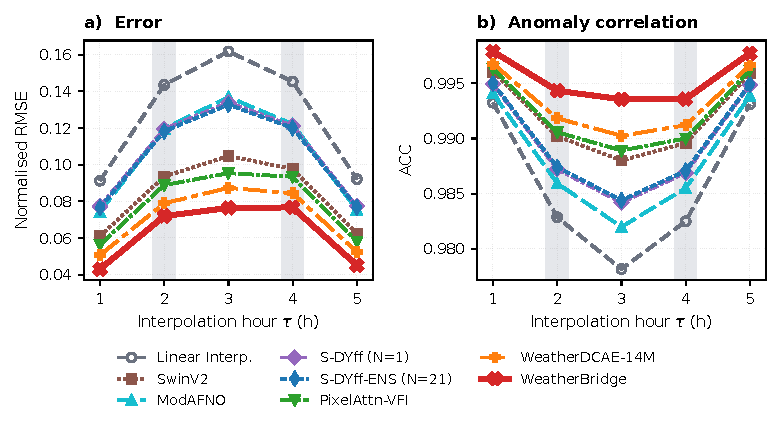
\includegraphics[width=\columnwidth]{images/fig_main_scores.pdf}
\caption{Full-year 2020 scores for the principal models.
\textbf{a)} Normalised RMSE. \textbf{b)} ACC against the WeatherBench-2
1990--2019 hourly climatology. WeatherBridge is the emphasized red curve.
Grey bands mark the held-out query hours
$\tau\in\{2,4\}$, which are absent from training. Curves share a window index;
tests use paired seven-day blocks. S-DYff and S-DYff-ENS use one and 21
stochastic reconstructions, respectively, from the same checkpoint.}
\label{fig:main_scores}
\end{figure}

\begin{table*}[t]
\centering
\caption{Performance at trained and held-out query hours on the 2020 ERA5 benchmark. Six-hour models train at $\tau\in\{1,3,5\}$ and hold out $\{2,4\}$; twelve-hour models hold out $\{4,6,8\}$. Entries are mean $\pm$ standard deviation of the 24-channel macro RMSE across query hours. The standard deviation describes variation between hours, not sampling uncertainty over dates. Differences between the trained and held-out columns also reflect the intrinsic difficulty of their query hours and are not an estimate of a generalisation gap.}
\label{tab:query-generalization}
\small
\setlength{\tabcolsep}{3.5pt}
\begin{tabular}{lrrrr}
\toprule
Model & 6 h seen & 6 h held out & 12 h seen & 12 h held out \\
\midrule
WeatherBridge & $\mathbf{0.055\pm0.019}$ & $\mathbf{0.074\pm0.003}$ & $\mathbf{0.099\pm0.033}$ & $\mathbf{0.133\pm0.008}$ \\
WeatherDCAE-14M & \underline{$0.063\pm0.021$} & \underline{$0.082\pm0.004$} & \underline{$0.107\pm0.034$} & \underline{$0.141\pm0.008$} \\
\midrule
\textit{Linear Interp.} & $0.115\pm0.040$ & $0.144\pm0.001$ & $0.202\pm0.074$ & $0.278\pm0.015$ \\
\bottomrule
\end{tabular}
\end{table*}


At the held-out hours of the six-hour task, WeatherBridge reaches RMSE
\WBSixHeldRMSE{}, $\WBSixHeldVsDCAEGainPct\%$ below WeatherDCAE-14M and
$\WBSixHeldVsLinearGainPct\%$ below Linear Interp. At the held-out hours of the
twelve-hour task, its RMSE is \WBTwelveHeldRMSE{}, improvements of
$\WBTwelveHeldVsDCAEGainPct\%$ and $\WBTwelveVsLinearHeldGainPct\%$ over the
same references. The gain over Linear remains close to the gain at trained
hours, and the model ordering persists at the held-out query hours.

A matched six-hour self-comparison measures the cost of withholding hours 2
and 4. Direct supervision lowers WeatherBridge RMSE at those hours by 8.77\%
in 2020 and 8.78\% in 2021; at trained hours 1, 3 and 5, the change is below
0.4\% (Supplementary Fig.~\ref{S-fig:full-query-summary}). Supplementary
Fig.~\ref{S-fig:full-query-field-hour} resolves the change by field and hour,
and Supplementary Table~\ref{S-tab:full-query-protocol} records which
checkpoint comparisons match both seed and update budget. The sparse-query
checkpoint transfers useful skill to both omitted hours; direct supervision
retains an 8.8\% advantage. This test covers integer hours, and the twelve-hour
setting lacks an all-query control.

Figs.~\ref{fig:fields_6h_thermodynamic},
\ref{fig:fields_6h_wind} and \ref{fig:fields_6h_mass_surface} resolve the
six-hour aggregate into the five interior-hour trajectories for every
evaluated field. WeatherBridge has
the lowest mean RMSE over $\tau=1,\ldots,5$ for 19 of 24 fields. WeatherDCAE-14M
remains better for the four geopotential levels and MSLP. WeatherBridge wins
most fields, but the mass-field regressions rule out a field-uniform claim.

The S-DYff-ENS curves add ensemble averaging to the same checkpoint and
evaluation windows. Supplementary Figs.~\ref{S-fig:supp_ens_12h_2021},
\ref{S-fig:supp_ens_6h_2022} and \ref{S-fig:supp_ens_12h_2022} complete the
field-wise comparison for twelve-hour interpolation in 2021 and both
intervals on the fixed 2022 sample. The ensemble-size comparison and its
paired single-draw control are described in Supplementary
Section~\ref{S-sec:sdyff-ensemble}.

\begin{figure*}[t]
\centering
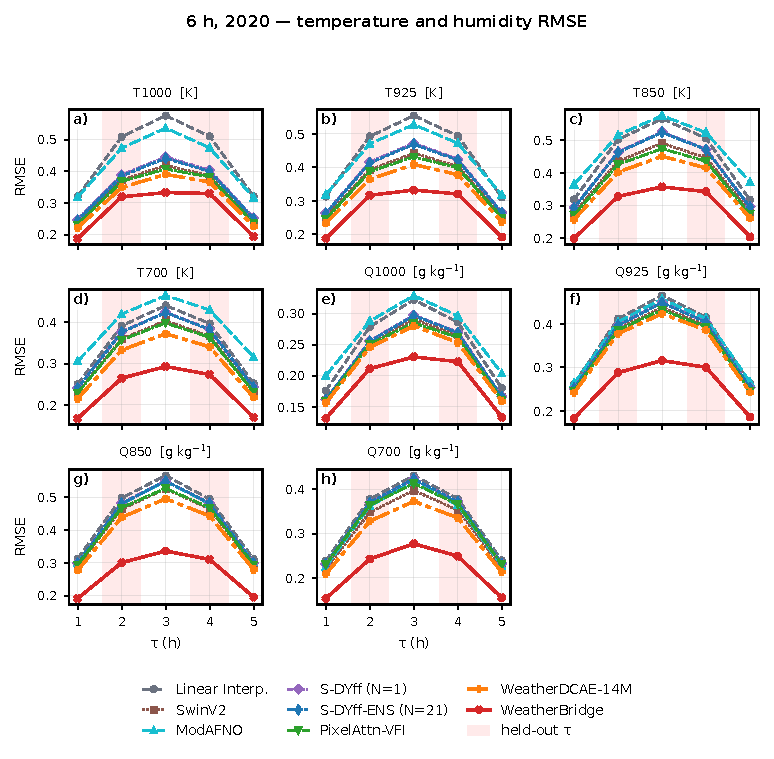
\includegraphics[width=0.96\textwidth,height=0.76\textheight,keepaspectratio]{images/fig_fields_6h_thermodynamic_phys.pdf}
\caption{Full-year 2020 physical-unit RMSE trajectories for temperature and
specific humidity at four pressure levels. Each panel follows the six-hour
interpolation from $\tau=1$ to 5\,h; lower is better. Pink bands mark held-out
query hours $\tau\in\{2,4\}$. WeatherBridge is the solid red curve. Scales
differ between fields and should only be compared within a panel. All neural
curves use the same evaluator and full-year window index.}
\label{fig:fields_6h_thermodynamic}
\end{figure*}

\begin{figure*}[t]
\centering
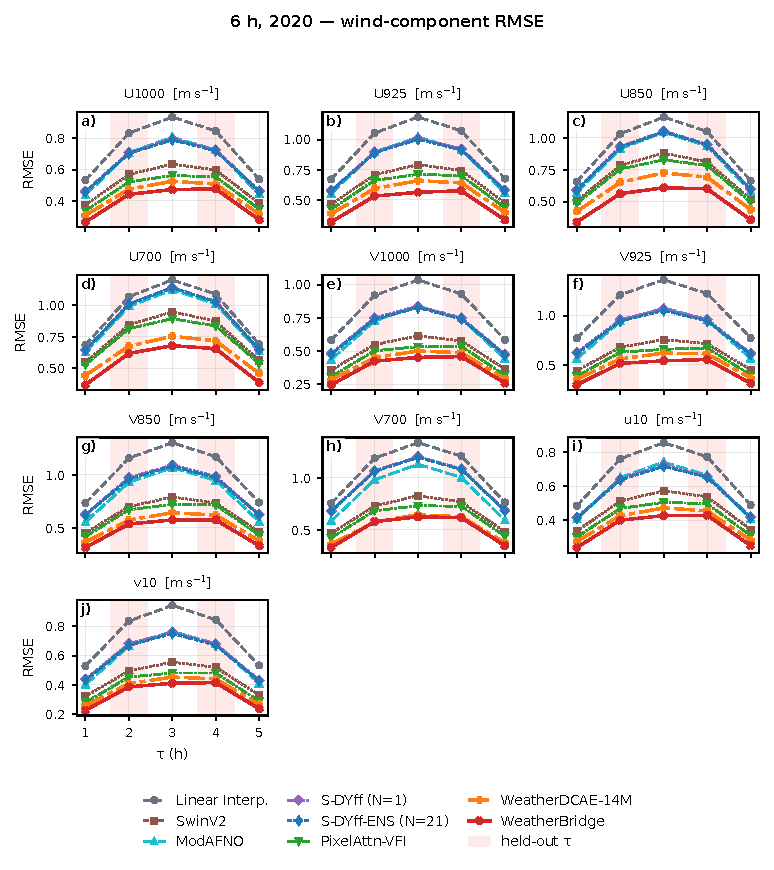
\includegraphics[width=0.96\textwidth,height=0.76\textheight,keepaspectratio]{images/fig_fields_6h_wind_phys.pdf}
\caption{Full-year 2020 physical-unit RMSE trajectories for zonal and
meridional wind at four pressure levels and 10\,m. Plotting conventions and
model provenance match Fig.~\ref{fig:fields_6h_thermodynamic}.}
\label{fig:fields_6h_wind}
\end{figure*}

\begin{figure*}[t]
\centering
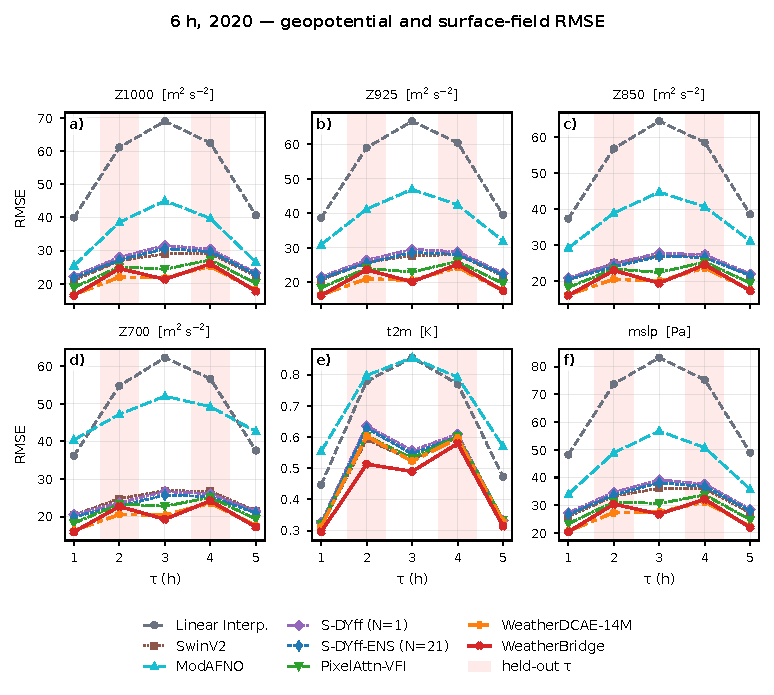
\includegraphics[width=0.96\textwidth,height=0.76\textheight,keepaspectratio]{images/fig_fields_6h_mass_surface_phys.pdf}
\caption{Full-year 2020 physical-unit RMSE trajectories for geopotential at
four pressure levels, 2-m temperature and mean sea-level pressure. Plotting
conventions and model provenance match
Fig.~\ref{fig:fields_6h_thermodynamic}.}
\label{fig:fields_6h_mass_surface}
\end{figure*}

\IfFileExists{postselection_2022.tex}{%
  The 2022 sample contains 48 disjoint 00 UTC windows on days 1, 8, 15 and 22 of
each month. We fixed this index before generating its predictions. The
comparison tests calendar transfer of both the all-hour aggregate and the
query hours omitted from optimisation.
\begin{table}[t]
\centering
\caption{Fixed 2022 comparison against WeatherDCAE-14M. Negative relative
differences favour WeatherBridge. Confidence intervals are for the paired
difference in mean normalised RMSE and use 10,000 seven-day block-bootstrap
draws.}
\label{tab:postselection-2022}
\small
\begin{tabular}{llrr}
\toprule
Horizon & Query hours & Relative $\Delta$ (\%) & 95\% CI for $\Delta$RMSE \\
\midrule
6 h & all & -12.62 & [-0.00887, -0.00839] \\
6 h & held out & -11.09 & [-0.00899, -0.00843] \\
12 h & all & -7.06 & [-0.00841, -0.00805] \\
12 h & held out & -5.69 & [-0.00823, -0.00779] \\
\bottomrule
\end{tabular}
\end{table}
All four upper confidence bounds are below zero. The result supports aggregate
and held-query calendar transfer. Ten six-hour and seven twelve-hour
field--hour cells nevertheless show Holm-significant regressions, so we make
no claim of universal dominance.
%
}{%
% The publication build requires the frozen calendar-transfer artifact.
}

Supplementary Figs.~\ref{S-fig:supp_channels_12h_body}--\ref{S-fig:supp_channels_12h}
report the corresponding 12-hour ablation without repeating the six-hour
panels above. Units and
climatological scales differ, so comparisons are meaningful within a field
and query hour, not across variables. Fig.~\ref{fig:main_scores}a gives the
normalised aggregate; Supplementary Figs.~\ref{S-fig:supp_ood2021_body}--\ref{S-fig:supp_ood2021_levels}
show the 2021 field ordering.

On the 2022 sample, WeatherBridge has lower pointwise RMSE in 109 of 120
six-hour and 254 of 264 twelve-hour field--hour cells. The paired aggregate
and held-out intervals in Table~\ref{tab:postselection-2022} exclude zero at
both gaps. Held-out RMSE is 11.09\% lower than WeatherDCAE-14M at six hours
and 5.69\% lower at twelve hours. The
internal Detail and Refine variants are 0.3--0.4\% better at 6\,h in 2020 and
2021, but WeatherBridge is better at 12\,h and has the lowest aggregate score
when the two gaps are considered together. Supplementary
Table~\ref{S-tab:architecture-ablation} reports that comparison.

The sample preserves the aggregate and held-out ordering while revealing
Holm-significant regressions in ten six-hour and seven twelve-hour field--hour
cells. The internal robustness sensitivity consequently retains
WeatherDCAE-14M; we report
that sensitivity analysis in Supplementary Table~\ref{S-tab:selector-diagnostics}
rather than using it to define the study's central held-out endpoint.
Supplementary Table~\ref{S-tab:vector-sht} gives representative vector-SHT
comparisons.

Same-checkpoint lesions show that both transport terms contribute to the
reported checkpoint. Disabling acceleration raises aggregate RMSE by 2.16\%;
disabling warped-anchor transport raises it by 60.54\% on the full-year 2020
index. Disabling the hydrostatic head has a smaller aggregate effect
(+0.04\%), but worsens all 25 targeted geopotential/MSLP field--hour cells
after Holm correction; mean hydrostatic-balance MSE rises by 1.06\% across the
five query hours (Supplementary Table~\ref{S-tab:component-lesions}). These
lesions test whether the trained checkpoint uses each term, not how a
model trained without that term would perform. The hydrostatic head has
a small field-specific effect, whereas transport accounts for the largest
checkpoint sensitivity. The fine, coarse and SFNO residual branches and
the learned blend gates are not isolated by these tests, so their individual
accuracy gains remain unquantified. The retrained Detail and Refine
variants change several mechanisms and do not resolve that attribution.
The 2021 comparison reuses the model set, normalisation, full-year window
construction and query-hour split from 2020; no checkpoint trains on 2021.
Because it informed development, the 2021 result is a calendar-transfer
diagnostic. The prespecified 2022 sample supplies the later calendar check. Supplementary
Table~\ref{S-tab:transfer-2021} reports its aggregate six-hour scores.

Exchanging the two anchors and replacing $t$ by $1-t$ produces a different
prediction. On the retained 48-endpoint diagnostic, WeatherBridge's
exchange RMSE is 0.287 in 2020 and 0.285 in 2021, more than three times its
forward reconstruction error (Supplementary Table~\ref{S-tab:anchor-exchange}).
The transport heads are bidirectional, while the complete interpolator is
asymmetric because the left and right endpoints retain different learned roles.

WeatherBridge improves on WeatherDCAE-14M at every UTC start in both years.
Its pooled advantage is $12.7\%$ within one assimilation window and $9.7\%$
across a boundary in 2020, with corresponding 2021 values of $12.6\%$ and
$9.6\%$ (Supplementary Table~\ref{S-tab:utc-start-strata}). Assimilation
timing changes the size of the gain, which nevertheless persists in all eight
year--start strata.

\subsection{Transfer to IFS HRES forecast trajectories}
\label{sec:hres_trajectories}

We replace the ERA5 anchors with two states from one IFS HRES forecast
trajectory and retain ERA5 as the intermediate target. For each anchor pair,
$\tau=1,\ldots,5$ denotes the offset inside the six-hour interval; forecast
lead is a separate coordinate. The resulting error combines temporal
interpolation with HRES--ERA5 mismatch.

\IfFileExists{hres_finetuning_results.tex}{%
  \subsubsection{Full-weight adaptation across forecast leads}
\label{sec:hres_finetuning}

Unlike the coefficient adapter below, this experiment updates the network
weights. Its 24-initialisation 2022 index is distinct from both the
16-initialisation coefficient-adapter test and the 48-window ERA5
calendar-transfer sample. The row labelled ``fine-tuned WeatherDCAE-14M'' in
Table~\ref{tab:hres-retrospective-2022} denotes full-weight optimisation, not
the WeatherBridge coefficient adapter.

Lead coverage was inspected on the 2021 development archive. Fine-tuning on
the short deployment range improves mean field--hour RMSE over linear
interpolation by $1.70\%$. Extending training to $0$--$216\,$h on a $24\,$h
lead grid raises the gain to $7.63\%$; using the native $6\,$h lead grid raises
it to $12.35\%$.

The two full-range checkpoints specialise by lead. Routing the coarse-grid
checkpoint below $48\,$h and the dense-grid checkpoint thereafter gives mean
RMSE 0.4671, compared with 0.5567 for Linear, 0.5143 for the coarse checkpoint
and 0.4880 for the dense checkpoint. Relative to each comparator, the routed
result improves by $16.10\%$, $9.18\%$ and $4.29\%$, respectively. These
development results define the routing rule but provide no confirmation
evidence.

On the fixed 2022 dates, the full-range coarse-grid checkpoint reduces
the mean of the 120 field--hour RMSE values from $0.2902$ to $0.2691$
($7.28\%$). The lead-routed ensemble reaches $0.2675$ ($7.83\%$), but its
spectral promotion audit is incomplete. We therefore retain the coarse-grid
checkpoint as the adapted model of record and report the ensemble as a
secondary result. Because the full-range branch postdates inspection of 2022,
these values are retrospective rather than independent confirmation evidence.

Statistical resampling uses the 24 forecast initialisations as blocks; the 600
window--hour records remain grouped within them.

\begin{table}[t]
\centering
\caption{Six-hour interpolation from IFS HRES forecast anchors to ERA5 on a
fixed 2022 retrospective set (24 initialisations; left-anchor leads
$\{0,24,48,72,96\}\,$h; right endpoint through $102\,$h). Scores are the
arithmetic mean of 120 latitude-weighted field--hour RMSE values. This index is
distinct from the coefficient-adapter and ERA5 calendar-transfer samples. The
lead-routed ensemble gives the lowest point estimate, but its spectral
promotion audit has not been run; bold therefore marks the
coarse-stride model of record, which passes the separately reported spectral
criterion. The full-range branch postdates inspection of 2022, so this table is
descriptive rather than independent confirmation.}
\label{tab:hres-retrospective-2022}
\begin{tabular}{lcc}
\toprule
Method & RMSE & vs.\ linear \\
\midrule
Linear interpolation                     & $0.2902$          & ---                 \\
WeatherBridge, no adaptation              & $0.2866$          & $+1.23\%$           \\
WeatherDCAE-14M, no adaptation            & $0.2876$          & $+0.91\%$           \\
WeatherDCAE-14M, short-range fine-tuned   & $0.2740$          & $+5.60\%$           \\
WeatherBridge, short-range fine-tuned     & $0.2711$          & $+6.59\%$           \\
\textbf{WeatherBridge, full-range coarse grid} & $\mathbf{0.2691}$ & $\mathbf{+7.28\%}$ \\
WeatherBridge, full-range dense grid      & $0.2715$          & $+6.45\%$           \\
WeatherBridge, lead-routed ensemble       & $0.2675$          & $+7.83\%$           \\
\bottomrule
\end{tabular}
\end{table}


The corresponding spectral audit covers Q850 and U850 at query hours 2 and 3
over spherical-harmonic degrees 80--180. The coarse-grid checkpoint satisfies
the predeclared shape and coherence margins in all four cells. The dense-grid
checkpoint fails, with coherence changes of $-0.038$ for Q850 and $-0.035$ for
U850 at query hour 2. The channels were selected during development, so this
audit can promote a checkpoint but cannot confirm performance on an
independently chosen spectral panel.

A final experiment isolates temporal reconstruction from forecast--analysis
mismatch by taking both anchors and the target from one HRES run. A twelve-hour
checkpoint reconstructs the archived six-hour state. On 16 initialisations,
WeatherBridge gives the lowest point estimate among the three evaluated neural
models, reducing RMSE by $42.6\%$ relative to linear interpolation
(Supplementary Table~\ref{S-tab:hres-same-trajectory} and Supplementary
Fig.~\ref{S-fig:hres-best-fields}).
This small 2021 sample is exploratory and has no training-seed uncertainty.
%
}{%
% The weight-adaptation results require the frozen fine-tuning artifacts.
}

\subsubsection{Frozen-coefficient adapter}

Before adaptation, Linear interpolation
has the lowest point estimate in 93 of 120 field--hour cells at 6\,h and 232
of 264 cells at 12\,h. Within the displayed three-model comparison,
WeatherDCAE-14M and WeatherBridge lead in 16/11 cells at 6\,h and 20/12 cells
at 12\,h, respectively.
The twelve-hour transfer scores and raw six-hour cell counts remain in
Supplementary Data~1, while Supplementary
Fig.~\ref{S-fig:nwp_adapter_2022} places the raw six-hour controls and the
fixed adapter on the 2022 test index. Nonlinear corrections learned
from ERA5 anchor pairs therefore transfer poorly to HRES anchors. The
validation-selected correction in Eq.~\ref{eq:nwp_adapter} addresses this
source shift. WeatherDCAE-14M and raw WeatherBridge are post-hoc controls; the
confirmatory adapter-versus-Linear test excludes both post-hoc curves.

Across the 16-initialisation 2022 test, the adapter reduces
aggregate RMSE from 0.73466 to 0.73382, a 0.114\% change. None of 10,000
sign-flip draws is at least as extreme as the observed effect (Monte Carlo
resolution $1/10001$); the paired MSE-effect 95\% interval is
$[0.00116,0.00129]$. Sign flips and bootstrap draws operate over the 16
forecast initialisations; the 3200 field--hour records remain grouped within
each initialisation. The reduction is
0.137\% at the held-out hours
$\tau\in\{2,4\}$, again with no exceedance in 10,000 sign flips. It is
concentrated at short HRES
leads: 2.384\% at 0--48 h and 0.301\% at 48--120 h, followed by the
predeclared exact tie at 120--240 h. Among the 72 active field--hour cells,
70 improve and two regress; the remaining 48 cells are exact guarded ties.
The two regressions are T700 at $\tau=2$
($-0.048\%$) and $\tau=4$ ($-0.028\%$). Thus aggregate and held-out-hour RMSE
improve despite two small T700 regressions.

The cell-centred SHT analysis in Supplementary
Table~\ref{S-tab:supp_nwp_spectra_2022} separates coefficient alignment from
amplitude error. The frozen
coefficient adapter increases high-wavenumber coherence and signed cospectrum for
both Q850 and U850 at $\tau\in\{2,3\}$. No sign-flip exceedance occurs in
the four field--hour cells; the two-test Holm family has resolution
$2/10001$. Energy and shape errors
are mixed: U850 shape improves at $\tau=2$, whereas three of four energy
comparisons and both Q850 shape comparisons favour Linear. Thus the adapter
improves alignment of small-scale coefficients but does not fully calibrate
their amplitude.

\IfFileExists{tab_sh_per_channel_12h_v6.tex}{%
\subsection{Spectral analysis}

Fig.~\ref{fig:weatherbridge_spectra_tau23} examines two six-hour query times:
$\tau=2$ was excluded from training, whereas $\tau=3$ was observed. We report
power ratio and signed cospectrum for Linear interpolation, the four neural
baselines, WeatherDCAE-14M and WeatherBridge.
Power can match despite misplaced or anti-phase
structure; a signed cospectrum near one also requires aligned coefficients.
Band-integrated energy, shape and phase statistics use every valid 2020 date
at the 00 and 12 UTC anchor starts, with paired calendar-week resamples.
Specific humidity (Q850) and zonal wind (U850) at 850\,hPa were chosen during
development to show moisture and wind behaviour and are interpreted
descriptively.

\begin{figure*}[t]
\centering
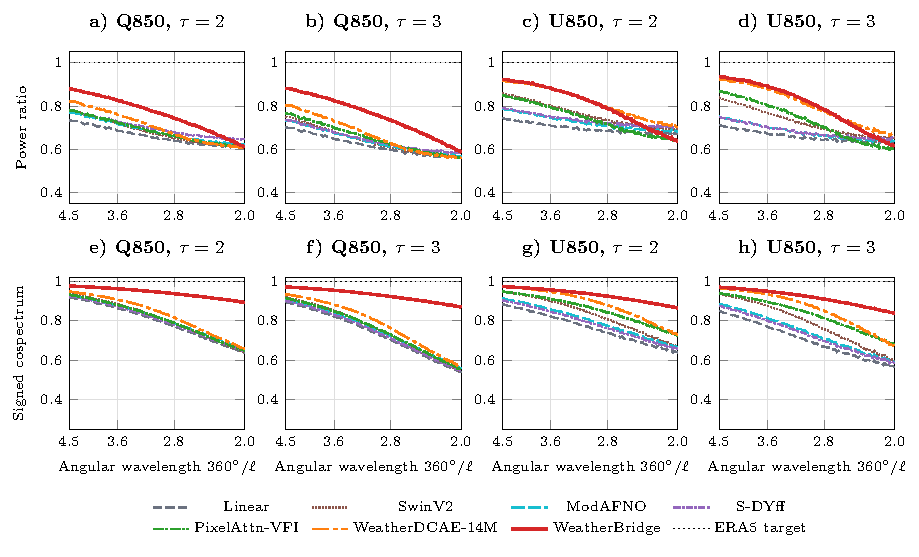
\includegraphics[width=0.96\textwidth]{images/fig_weatherbridge_spectra_tau23.pdf}
\caption{Six-hour spherical-harmonic diagnostics at a held-out query hour
($\tau=2$) and a trained hour ($\tau=3$). Panels \textbf{a)--d)} show power
ratio; panels \textbf{e)--h)} show signed normalised cospectrum for Q850 and U850
over $\ell\in[80,180]$; one is ideal. Curves use all valid 2020 dates at
00 and 12 UTC anchor starts under the SHT protocol defined in Methods.
WeatherBridge is red throughout the paper; the other model colours match the
RMSE and ACC figures.}
\label{fig:weatherbridge_spectra_tau23}
\end{figure*}

WeatherBridge has the highest signed cospectrum among the plotted methods in
all four Q850 and U850 panels, while the power-ratio ordering varies with field,
wavenumber and query hour. Power and cospectrum must be read together: similar
amplitude can coexist with weaker phase alignment. The all-field
spectral tests determine the broader comparison.
Supplementary Fig.~\ref{S-fig:supp_spectra_12h} shows the corresponding 12\,h
power ratios for Q850 and V850 at a trained hour ($\tau=5$) and a held-out
hour ($\tau=6$).
The figure shows the component curves. The scalar and vector
spherical-harmonic-transform (SHT) summaries in Supplementary
Tables~\ref{S-tab:sh_per_channel_6h} and
\ref{S-tab:sh_per_channel_12h} determine the spectral comparison.
}{%
% Numerical spectral results are inserted only after schema-v6 validation.
}

% Section: 12h interval-length ablation.
\subsection{Twelve-hour interval-length ablation}
\label{sec:12h}

To test sensitivity to anchor spacing without redefining the primary task, we
double the six-hour anchor gap.
All 12\,h variants use the same 24 channels, 2017--2019 training years and
query coordinate $t=\tau/\Delta$. They train at
$\tau\in\{1,2,3,5,7,9,10,11\}$ and are evaluated at every interior hour.
The held-out hours $\{4,6,8\}$ include the midpoint and test interpolation
between sampled query times. The learned path between those discrete hours
remains unobserved. Methods gives model capacities and update budgets.

\IfFileExists{main_metrics_v2.tex}{%
Supplementary Figs.~\ref{S-fig:supp_channels_12h_body} and
\ref{S-fig:supp_channels_12h} report the 12\,h result by channel class.
WeatherBridge is evaluated at all eleven interior hours using the same
normalisation as the other models. It obtains mean
RMSE$_{\text{norm}}=\WBTwelveRMSE$ over the full grid and
$\WBTwelveHeldRMSE$ on the held-out hours, compared with
$\WBTwelveLinearRMSE$ and $\WBTwelveLinearHeldRMSE$, respectively, for
Linear Interp. Its mean ACC is $\WBTwelveACC$ over all hours and
$\WBTwelveHeldACC$ on
the held-out subset. The per-field panel cannot isolate the source of an error
at a held-out hour; the spatial backbone, optimisation and capacity also
change across models. Off-scale ModAFNO values are marked explicitly in the
Supplementary panel.

\IfFileExists{tab_main_12h_v2.tex}{%
Supplementary Table~\ref{S-tab:main-12h} reports the aggregate 12\,h
held-out-hour comparison for the 2020 development year. All
learned models use the same nominal $0.5^\circ$ data split, query-hour sampler,
peak learning rate and evaluation windows; their architecture-specific update
counts are reported in Supplementary Table~\ref{S-tab:protocol_summary}.
}{% The aggregate table is inserted only after matched-v2 validation.
}
\IfFileExists{tab_sh_per_channel_12h_v6.tex}{%
The full-year spherical-harmonic audit is reported by channel
in Supplementary Table~\ref{S-tab:sh_per_channel_12h}. The corresponding
6\,h results appear in Supplementary Table~\ref{S-tab:sh_per_channel_6h};
both tables use the block-average latitude coordinates
with spherical strip-area quadrature and retain every valid date on the
00/12 UTC start-time index. At 12\,h, WeatherBridge preserves less mean
high-frequency energy than WeatherDCAE-14M ($0.768$ versus $0.793$) and is
farthest from unity for T700 and T2m. The advantage observed in selected
six-hour phase diagnostics therefore does not extend uniformly to the longer
interval.%
}{%
% Per-channel spectral tables are inserted only after schema-v6 validation.
}

}{% The validated 12 h figure and tables are inserted as one artifact set.
}

\IfFileExists{tab_downstream_physics_v2.tex}{%
\subsection{Diagnostic physical balances}
\label{sec:physics_results}

Pointwise accuracy does not guarantee that a reconstructed state has the
same diagnostic balance as ERA5. Supplementary Table~\ref{S-tab:physics_balance} reports
the predicted-to-ERA5 ratio for the ageostrophic-wind RMSE and the
hydrostatic residual. Each entry averages the interior query hours and
180 anchor windows selected uniformly from a 48-hour candidate grid in
2020. WeatherBridge is shown beside WeatherDCAE-14M and linear interpolation.
A ratio of one reproduces the ERA5 residual scale. Values below one may result
from smoothing, so neither the minimum nor the maximum ratio is preferred;
distance from one is the relevant quantity. This smaller balance audit is
descriptive; the separate full-year physical suite in Methods supplies the
paired robustness analysis.

}{% The validated diagnostic-balance table is mandatory for publication.
}

\IfFileExists{tab_downstream_diurnal_v2.tex}{%
\subsection{Regional diurnal-cycle reconstruction}
\label{sec:diurnal_results}

Global RMSE leaves regional timing and amplitude unresolved. We therefore
aggregate T2m, U10 and V10 over four predefined regions and 12 monthly local-time
climatologies. Supplementary Table~\ref{S-tab:diurnal} gives equal weight to each of the
resulting 144 region--month--field strata and compares the same three methods
as the balance audit. The amplitude statistic measures departure
from the ERA5 climatological range, while the circular peak error measures
local-time displacement. These descriptive regions expose local behaviour
that global RMSE misses; they were excluded from model selection and provide
no population-level regional inference.

}{% The validated regional-diurnal table is mandatory for publication.
}

\begin{deferreddiscussion}
\section{Discussion}
\label{sec:discussion}

Learned corrections remain useful at sampled query hours omitted from
optimisation. WeatherBridge retains its aggregate lead at the held-out hours
for both six- and twelve-hour anchor gaps. On the 2022 ERA5 sample,
held-out RMSE is 11.09\% and 5.69\% below WeatherDCAE-14M, respectively.
The matched six-hour control quantifies the cost of withholding supervision:
restoring hours 2 and 4 to training lowers their RMSE by about 8.8\%, while
changing trained-hour RMSE by less than 0.4\%. The sparse-query model transfers
useful skill, while direct supervision remains better. The evidence covers
integer query hours; continuous-time evaluation and a matched twelve-hour
control remain open.

WeatherBridge assigns different roles to transport and residual synthesis.
The flow heads move resolved structure toward the requested hour; the local
and global residual branches model deformation, unresolved development and
smooth mass-field change. Removing acceleration from the trained checkpoint
raises aggregate RMSE by 2.16\%, and removing warped-anchor transport raises
it by 60.54\%. The hydrostatic head has a much smaller aggregate effect, but
improves every geopotential/MSLP field--hour cell that it modifies and reduces
mean hydrostatic-balance error. These internal displacements improve the
prediction but represent neither observed parcel tracks nor conservation
constraints.

Spectral power alone cannot distinguish a correctly placed front from one
with the right amplitude at the wrong longitude. At six hours WeatherBridge
improves signed cospectrum in several high-wavenumber diagnostics, while its
power-ratio error depends on the field and query hour. At twelve hours
WeatherDCAE-14M retains more mean band energy, including clear advantages for
T700 and T2m. The spectral loss therefore improves selected coefficient
alignment without calibrating small-scale amplitude across both anchor gaps.

The IFS HRES experiments expose a second boundary. ERA5-trained corrections
transfer poorly when both anchors come from a forecast trajectory. A
coefficient adapter gives only a 0.114\% aggregate gain, whereas full-weight
adaptation across the deployed forecast-lead range gives 7.28\% on the
24-initialisation 2022 audit. That number is retrospective because the
full-range branch was designed after 2022 had been inspected. It also combines
temporal reconstruction with correction of systematic forecast error;
correlated endpoint and interior errors prevent an additive decomposition. An
independent forecast archive is therefore needed before treating 7.28\% as a
prospective deployment estimate.

The physical and regional diagnostics add information that pointwise RMSE
misses. Smoothing can reduce ageostrophic or hydrostatic residuals without
matching the ERA5 balance, and four regional diurnal climatologies can expose
local-time phase errors. The regions are descriptive examples. The separate
robustness audit also records fieldwise, spectral, physical and
temporal-curvature regressions. The resulting claim concerns aggregate
interpolation at held-out hours with documented local regressions.

\end{deferreddiscussion}

\begin{deferredmethoddetails}
\subsection{Implementation and compute}
\label{app:impl}
Runs use PyTorch~2.5.1, CUDA~12.4, PyTorch Lightning~2.6.1 and
\texttt{torch-harmonics}~0.7.3 with mixed precision. The 12\,h ModAFNO follows
the official \texttt{physicsnemo} reference; the compact 6\,h variant uses our
implementation. Training and evaluation use two NVIDIA A100-80GB SXM4 GPUs
and a 486~GiB host-memory allocation. Supplementary
Tables~\ref{S-tab:protocol_summary} and \ref{S-tab:hyperparams} report the
per-model training budgets, parameter counts and architecture settings.

Inference latency is the median of seven CUDA-event repeats, each containing
20 bfloat16 forward passes after five warm-ups, on one A100-80GB at batch size
one and $24\times360\times720$ resolution. The benchmark uses random-input
seed 2027, cycles $t\in\{0.25,0.50,0.75\}$ and compares every candidate with
the fastest model measured in the same process.

\end{deferredmethoddetails}



\subsection{Event-scale evaluation under atmospheric extremes}
\label{sec:extreme_events}

Independent reports defined six events before error inspection: the Texas
cold outbreak, Pacific Northwest heatwave, Hurricane Ida, and Typhoons
Surigae, Chanthu and Rai. The evaluation manifest records their regions and
diagnostic fields. Six cases are too few to estimate an
extreme-event climatology. They do test whether the aggregate 2021 ordering
survives in high-impact local states without fine-tuning or test-time
adaptation. The aggregate summary below covers all six events.
Fig.~\ref{fig:extreme_events} shows three cyclone cases selected by the rule
stored in the figure provenance.

\begin{figure*}[t]
\centering
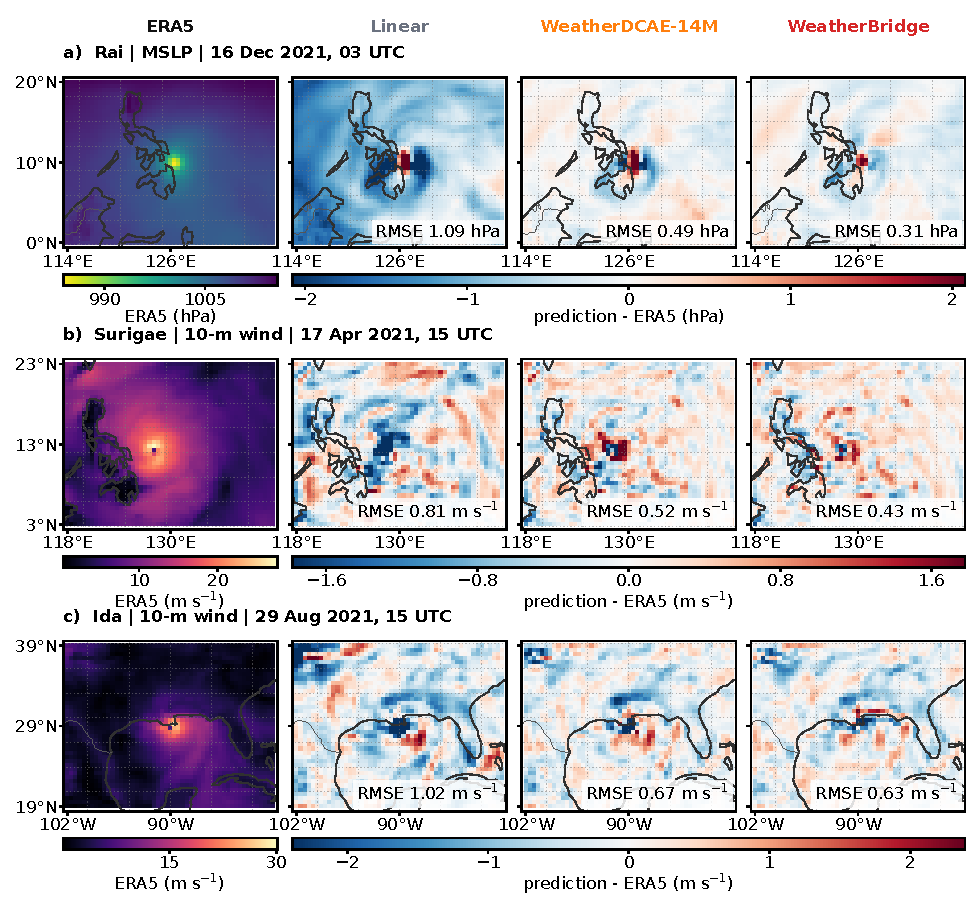
\includegraphics[width=0.96\textwidth]{images/fig_extreme_events_2021.pdf}
\caption{Local diagnostics for three cases from the independently selected
2021 extreme-event set. In panels \textbf{a)--c)} the leftmost column is ERA5
and the remaining three columns are the signed error of Linear Interpolation,
WeatherDCAE-14M and WeatherBridge at $\tau{=}3$\,h for Typhoon Rai mean
sea-level pressure, Typhoon Surigae 10-m wind speed and Hurricane Ida 10-m
wind speed.
Error maps share a colour range within each row, and annotations give
area-weighted RMSE over the displayed region. Maps are illustrative post-hoc
diagnostics: from the four cyclone candidates they retain cases with lower
WeatherBridge RMSE than WeatherDCAE-14M for the displayed
field and hour. Aggregate results in the text retain all six events, including
Chanthu.}
\label{fig:extreme_events}
\end{figure*}

\IfFileExists{extreme_event_metrics_v1.tex}{%
% Auto-generated by scripts/make_fig_extreme_events.py.
\newcommand{\WBExtremeEventCount}{6}
\newcommand{\WBExtremeEventWins}{6}
\newcommand{\WBExtremeMeanRMSE}{0.087}
\newcommand{\DCAEExtremeMeanRMSE}{0.097}
\newcommand{\LinearExtremeMeanRMSE}{0.144}
\newcommand{\WBExtremeRelativeGain}{10.5}
\newcommand{\WBExtremeWindRMSE}{0.449}
\newcommand{\DCAEExtremeWindRMSE}{0.482}
\newcommand{\WBExtremeWindRelativeGain}{6.8}

WeatherBridge has lower event-aggregate RMSE in
\WBExtremeEventWins{}/\WBExtremeEventCount{} cases. Its mean normalised RMSE is
\WBExtremeMeanRMSE{}, compared with \DCAEExtremeMeanRMSE{} for WeatherDCAE-14M
and \LinearExtremeMeanRMSE{} for Linear Interpolation, a
\WBExtremeRelativeGain\% reduction relative to WeatherDCAE-14M. Across the four
tropical cyclones, the corresponding wind-speed RMSEs are
\WBExtremeWindRMSE{} and \DCAEExtremeWindRMSE\,m\,s$^{-1}$, respectively, a
\WBExtremeWindRelativeGain\% reduction.
}{% Numerical event claims require the provenance-bound extreme-event artifact.
}
WeatherDCAE-14M has the smaller maximum-wind error in three of the four
cyclones and the smaller temperature-extremum error in both temperature cases.
WeatherBridge has lower error over the surrounding event fields. The models
therefore rank differently for distributed accuracy and isolated peak
retention.

Fig.~\ref{fig:haishen_case} adds a development-year trajectory rather than a
single selected hour. It shows mean sea-level pressure during Typhoon Haishen
at three consecutive query times, including both held-out hours. Supplementary
Fig.~\ref{S-fig:supp_laura_wind} gives the corresponding vector-wind comparison
during Hurricane Laura. Both are development-time qualitative diagnostics;
the 2021 event audit excludes them.

\begin{figure*}[t]
\centering
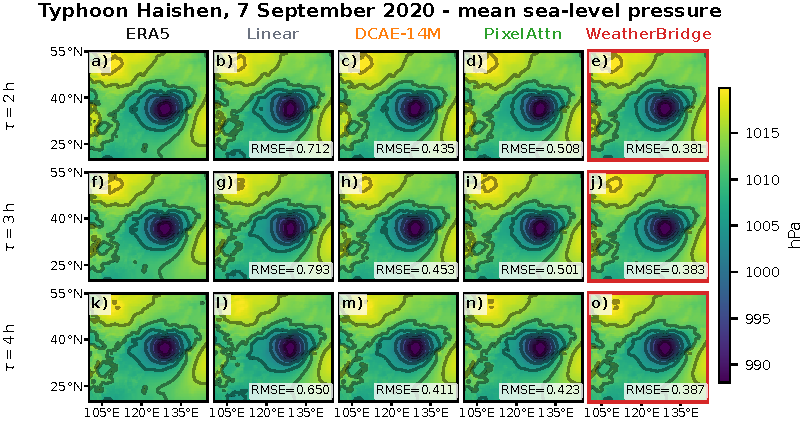
\includegraphics[width=0.96\textwidth]{images/fig_haishen_mslp.pdf}
\caption{Mean sea-level pressure reconstruction during Typhoon Haishen on
7 September 2020. Columns show ERA5, Linear Interpolation,
WeatherDCAE-14M, PixelAttn-VFI and WeatherBridge; rows show
$\tau=2,3,4$\,h. The second and fourth hours were excluded from training.
Annotations report RMSE over the fixed $25{-}48^\circ$N,
$115{-}145^\circ$E evaluation box.}
\label{fig:haishen_case}
\end{figure*}

% Discussion follows the complete Results section in the npj Article order.
\deferreddiscussionbody


All models are trained against ERA5, whose hourly sequence contains
assimilation increments as well as atmospheric evolution
\cite{ingstad2026hourglass}. The 2021 audit changes the calendar year while
retaining the data source, and the IFS HRES experiment covers a bounded set of
forecast anchors. Native Pangu-Weather, GraphCast and other data-driven
forecast trajectories remain untested because their grids, variable sets and
source-specific errors require a separate transfer experiment. ERA5-relative accuracy
may also reproduce the spatially varying observational constraints of the
reanalysis.

The spatial conclusions apply to the stored nominal $0.5^\circ$ grid.
Evaluation uses the actual block-average strip areas, and the spectral
diagnostics apply a spherical-harmonic transform at those coordinates. The
transport trunk itself is a latitude--longitude network with circular padding
in both tensor dimensions. Periodicity is correct in longitude but creates an
artificial adjacency between the northernmost and southernmost rows. Only the
low-wavenumber SFNO correction operates in a spherical-harmonic basis. A
pole-aware trunk, such as a cubed-sphere convolutional network
\cite{weyn2020dlwp}, would require matched retraining.

WeatherBridge is a deterministic 24-field interpolator for six-hour anchor
gaps; the twelve-hour experiment tests sensitivity to a longer interval. Its
evaluated scope ends at the later anchor and covers neither predictive
uncertainty, precipitation nor $0.25^\circ$ resolution. Architecture-specific
paper-scale schedules support a quality comparison, not matched-compute or
asymptotic rankings. The present checkpoint supports retrospective gap filling
on a finer temporal grid; warnings, aviation routing and other safety-critical
decisions lie outside its evaluated scope.
Squared-error optimisation targets a conditional mean
\cite{gneiting2011point}; low RMSE is therefore insufficient evidence of
realistic conditional variability. Evaluating a probabilistic interpolator
would additionally require a sampling protocol and proper scores such as
CRPS \cite{gneiting2007proper}.

\deferredmethodsintrobody
\deferredmethodsrestbody
\deferredmethoddetailsbody

\subsection{Physical-consistency diagnostics}
\label{sec:physics_diagnostics}

A full-year per-window diagnostic suite complements the smaller balance table
in Results. It contains normalised
MSE for horizontal wind divergence, relative vorticity and kinetic energy;
MSE between predicted and ERA5 hydrostatic residuals; area-weighted negative
specific-humidity fraction; absolute relative global MSLP bias; and absolute
relative lower-tropospheric moisture bias. Divergence and vorticity use
spherical finite differences and exclude latitudes poleward of
$75^\circ$; all other reductions use the declared strip areas. Every
quantity is non-negative and lower is better. These values are stored for
each full-year evaluation window and compared with paired seven-day blocks.

The smaller balance audit uses uniformly spaced windows and measures two
residual magnitudes; the robustness audit evaluates all seven physical
diagnostics. Geostrophic wind is derived from the horizontal
geopotential gradient at 850 and 700\,hPa using centred spherical finite
differences. We then compute the latitude-weighted RMSE
of the ageostrophic residual over $15^\circ$--$70^\circ$ absolute
latitude. Hydrostatic consistency is measured on the adjacent
1000/925/850/700\,hPa layers using
$\Delta Z+R_d\overline{T_v}\Delta\ln p$, where
$T_v=T(1+0.61q)$, and is normalised by the ERA5 residual from the same
windows. Both diagnostics use the declared spherical strip areas of the stored
block-average grid. These diagnostics are evaluated for both
6\,h and 12\,h anchor spacings at every interior query hour. We select 180
start times uniformly from the 2020 48-hour candidate grid and reuse the
exact index for every model within a horizon. None of these quantities enters
the training loss.

\subsection{Diurnal-cycle diagnostic}

We reconstruct hourly T2m, U10 and V10 sequences to test regional timing and
amplitude independently of global RMSE. Diurnal amplitude and peak hour are
evaluated in predefined
$5^\circ$ boxes over the Sahel, Amazon, Congo and south-eastern
Australia. The diagnostic reports amplitude bias and circular peak-time
error relative to ERA5 for all four compared methods. We average each
error equally over four regions, 12 calendar months and three surface
fields, giving 144 strata per model and horizon. The amplitude statistic
is $|A_{\mathrm{recon}}/A_{\mathrm{ERA5}}-1|$; peak-time error is
$\min(|\Delta h|,24-|\Delta h|)$.

\subsection{Reproducibility and statistical analysis}
\label{sec:reproducibility}

Linear interpolation and learned models use identical anchor pairs. In the
principal architecture comparison, 95\% intervals for aggregate RMSE use
$B{=}5000$ paired bootstrap draws over contiguous seven-day blocks of
the common full-year index. Block resampling preserves local temporal
dependence \cite{kunsch1989jackknife}; independent resampling of hourly
fields would disregard that dependence. Calendar splits address a separate
problem: leakage between temporally related training and evaluation data
\cite{roberts2017crossvalidation}. Pairing is retained within each draw, and
the channel set and all query hours remain grouped with their
anchor block. The full-year tests contain 53 calendar-week blocks. Sparse
hard-window subsets retain 19--30 non-empty blocks, with the exact
\texttt{n\_blocks} deposited for each comparison; draws lacking any requested
query hour are discarded and redrawn; the output artifact records the number
discarded.

The six-hour full-query control uses the same 2014--2019 training pool,
anchor construction, 24 fields and full-year 2020/2021 evaluation windows
as the sparse-query runs. For WeatherBridge, seed, optimiser-step budget,
effective batch size, precision and loss weights are matched; the training
query set changes from $\{1,3,5\}$ to $\{1,2,3,4,5\}$ h. Its paired
sparse-minus-full RMSE intervals use 5,000 day-block bootstrap draws,
rather than the seven-day blocks of the principal comparison. They measure
evaluation-period variability for one matched training seed. The other
architectures have unequal or incompletely documented seeds or update
budgets (Supplementary Table~\ref{S-tab:full-query-protocol}) and are
reported as diagnostic comparisons.

Mixed-precision kernels and cuDNN operations prevent bit-exact
reproduction. The intervals quantify test-period sampling variability.
Training sensitivity is reported through three paired seed-to-seed
forecast-anchor comparisons, which provide paired effects rather than a
distributional seed-level interval.

Supplementary Data~1 gives the observed effect, 95\% interval and block-swap
permutation $p$ value for every inferential comparison in the robustness
audit. Aggregate tests are two-sided; cellwise improvement and regression
tests are one-sided. The significance threshold is $\alpha=0.05$ after
correction within each family. Cellwise families retain both raw and
Holm--Bonferroni-adjusted values \cite{holm1979simple}, together with effect
directions. Raw Monte Carlo $p$ values use the plus-one
estimator $(r+1)/(B+1)$. Values at $1/(B+1)$ mean that no resampled statistic
was as extreme as the observation; they are marked
\texttt{p\_censored=true} instead of being printed as exact tail probabilities. The study
was not preregistered.

Field--hour RMSE, upper-5\%-hard-window RMSE and ACC each form a separate
family of $24(\Delta-1)$ tests for each candidate, horizon and year, with
$\Delta$ expressed in hours. Temporal curvature forms a 24-field family;
physical tests are corrected across the named diagnostics; each scalar and
vector spectral metric is corrected across its query-hour--field grid.
The 2020 and 2021 families are kept separate.
The internal robustness sensitivity rejects a candidate with any
Holm-significant regression in these families against WeatherDCAE-14M.
It also requires at most 15 million parameters, latency no greater than
1.25 times the fastest candidate, non-increasing aggregate and held-out
RMSE, and paired IFS HRES improvement in at least two of three seeds with
a non-positive mean change. This rule was fixed after development on 2020
and inspection of 2021. Supplementary Information reports its outcomes
separately from the primary aggregate comparison.
This familywise accounting avoids interpreting isolated significant
field--hour cells as independent confirmations \cite{wilks2016stippled}.

\subsection{Use of generative AI}

Generative AI tools assisted with language editing and translation,
manuscript revision, and preparation of code and figure layouts. Weather
fields and reported metrics come from the datasets and model evaluations
described in Methods. The authors are responsible for the code, analyses,
figures, references and conclusions in the final manuscript.

\backmatter

\bmhead{Data availability}

ERA5 is available from the Copernicus Climate Data Store
(\url{https://cds.climate.copernicus.eu/}) and through the
WeatherBench-2 archive
(\url{https://console.cloud.google.com/storage/browser/weatherbench2/}).
The IFS HRES audit uses the WeatherBench-2 HRES archive
(\url{https://console.cloud.google.com/storage/browser/weatherbench2/datasets/hres/}).
Methods specifies the $0.5^\circ$ product, splits, normalisation and channel
set. Supplementary Data~1 reports paired effects, intervals, $p$ values and
source hashes. Supplementary Data~2 contains the prespecified 2022 WeatherBridge
assessment and binds it to the evaluation index, verified memmap and model
manifest by SHA-256.

\bmhead{Code availability}

\IfFileExists{code_archive_statement.tex}{%
  Source code, experiment configurations, figure-generation scripts and
seven trained checkpoints are available at
\url{https://github.com/dsuhoi/weatherbridge}
\cite{sukhorukov2026weatherbridgecode}.
The versioned snapshot includes metric summaries, normalisation, static
fields and an example ERA5 window; weights are distributed through Git LFS.
It provides WeatherBridge at 6 h and 12 h intervals and the five learned
6 h comparators. Other 12 h comparator, full-query control and HRES-adapted
checkpoints are not included.
Full-year inference requires the external datasets described above;
redrawing figures from stored scores does not rerun inference.
%
}{%
The review package contains the training, evaluation and figure-generation
code, including the canonical WeatherBridge configuration
and environment metadata, provenance manifests and checkpoint hashes. The
review package also records the configuration of each evaluated checkpoint.
\PackageWarning{weatherbridge}{Public code and checkpoint archive statement
  requires author confirmation before submission}
}

\bmhead{Acknowledgements}

Computations were performed on the Cloud.ru SR006 infrastructure and the
Fibonacci research cluster.

\IfFileExists{funding_statement.tex}{%
  \parThis study received no funding.
%
}{%
\PackageWarning{weatherbridge}{Funding statement requires author confirmation
  before submission}
}

\bmhead{Author contributions}

D.S. led the study, implemented the models and evaluation protocol,
performed most of the experiments and analyses, prepared the main figures,
and wrote and revised the manuscript. A.Z. implemented and conducted the
full-query-hour ablation experiments and prepared the corresponding figures.
Y.M., I.M. and I.O. supervised the study, contributed to the development and
discussion of the research ideas, and revised the manuscript. All authors
discussed the results and approved the final manuscript.

\bmhead{Competing interests}

The authors declare no competing interests.

\bibliography{references}

\end{document}
